\documentclass[hidelinks,12pt,a4paper,openright,twoside]{book}
\usepackage[italian]{babel}
\usepackage[utf8]{inputenc}
\usepackage{fourier}

% To avoid GitHub Action error
\usepackage{hyperref}

% Images
\usepackage{graphicx}
\usepackage{caption}
\usepackage{subcaption}
\usepackage{float}
\graphicspath{ {../Images} }

% Stop hyphenation
\usepackage[none]{hyphenat}

% Background page image.
\usepackage{eso-pic}
\usepackage[top=2cm, bottom=2cm, outer=0cm, inner=0cm]{geometry}

% To hide images
\usepackage[allfiguresdraft]{draftfigure}

% To color text parts
\usepackage{xcolor}

% Minipages in the same line
\usepackage{tabularx}

% License
\usepackage[
type={CC},
modifier={by-nc-sa},
version={4.0},
]{doclicense}

\begin{document}
	
	% Remove page number
	\pagestyle{empty}
	
	% Album Cover
	\begin{center}
		\vspace*{15mm}
		\fboxrule=4pt{
		\fbox{ %                  height                                width
			\begin{minipage}[l] [\dimexpr 0.150\textwidth \relax] [t] {\dimexpr .460\textwidth \relax}
				\vspace{5mm}
				\centering{\large \textbf{Album sulle opere dei Musei Civici\\}}
				\bigskip
				Alice Balestieri \\
				Francesco Rombaldoni
			\end{minipage}
			}
		}
	\end{center}
	
	% Background image
	\AddToShipoutPictureBG*{\includegraphics[draft=false, width=\paperwidth,height=\paperheight]{example-image}}
	\newpage
	
	%--------- Page 1 ----------
		
	%First line
	\hspace{5mm}{
	\begin{tabularx}{\textwidth}{XX}
		{
			\hspace{2mm}
			%  Mengaroni_Ferruccio-Medusa
			\setdf{content={\textcolor{white}{\hspace{25mm} \Large \#1}}}
			\colorbox{black}{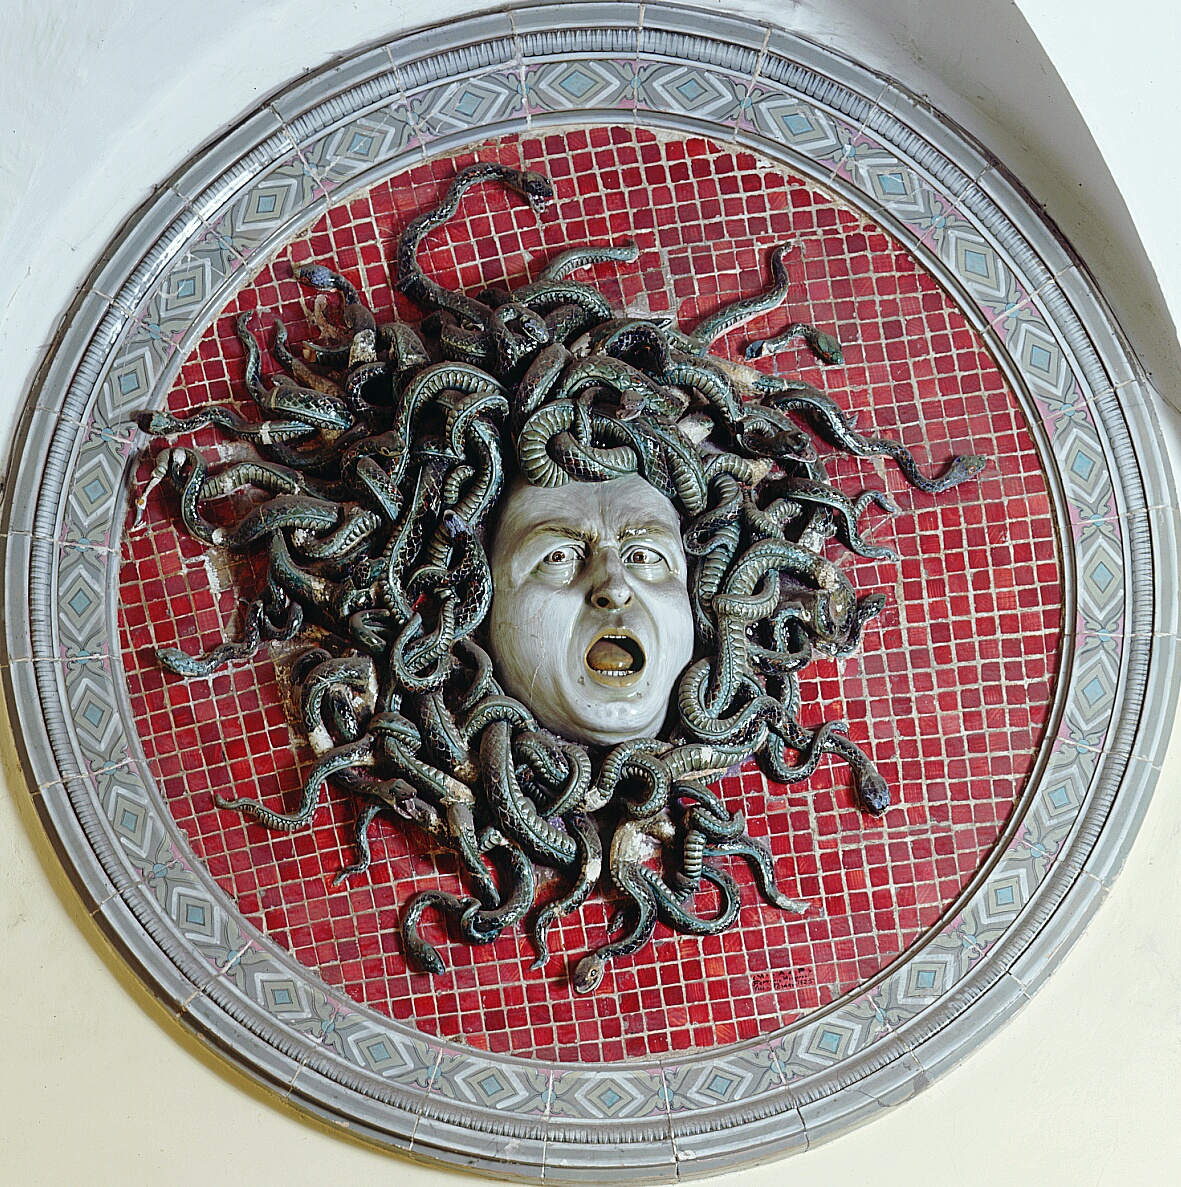
\includegraphics[scale = 1.2]{Mengaroni_Ferruccio-Medusa.jpg}}
			\bigskip
			\newline
			\begin{minipage}{0.8\linewidth}
				\raggedright
				"La Medusa" accoglie i visitatori introducendoli alle sale espositive; si tratta dell'ultima opera di Ferruccio Mengaroni.\\
				L'imponente Medusa ritrae i lineamenti dell'artista pesarese: la leggenda narra che, per riprodurre il proprio volto, egli si fosse servito di uno specchio che poi si ruppe.
			\end{minipage}
		}&{}
	\end{tabularx}
	}

	% Second line
	\vspace{5mm}
	\nopagebreak
	\begin{tabularx}{\linewidth}{XX}
		{}&{
			% Bellini_Giovanni-Incoronazione_della_Vergine
			\hspace{3mm}
			\setdf{content={\textcolor{white}{\hspace{25mm} \Large \#2}}}
			\colorbox{black}{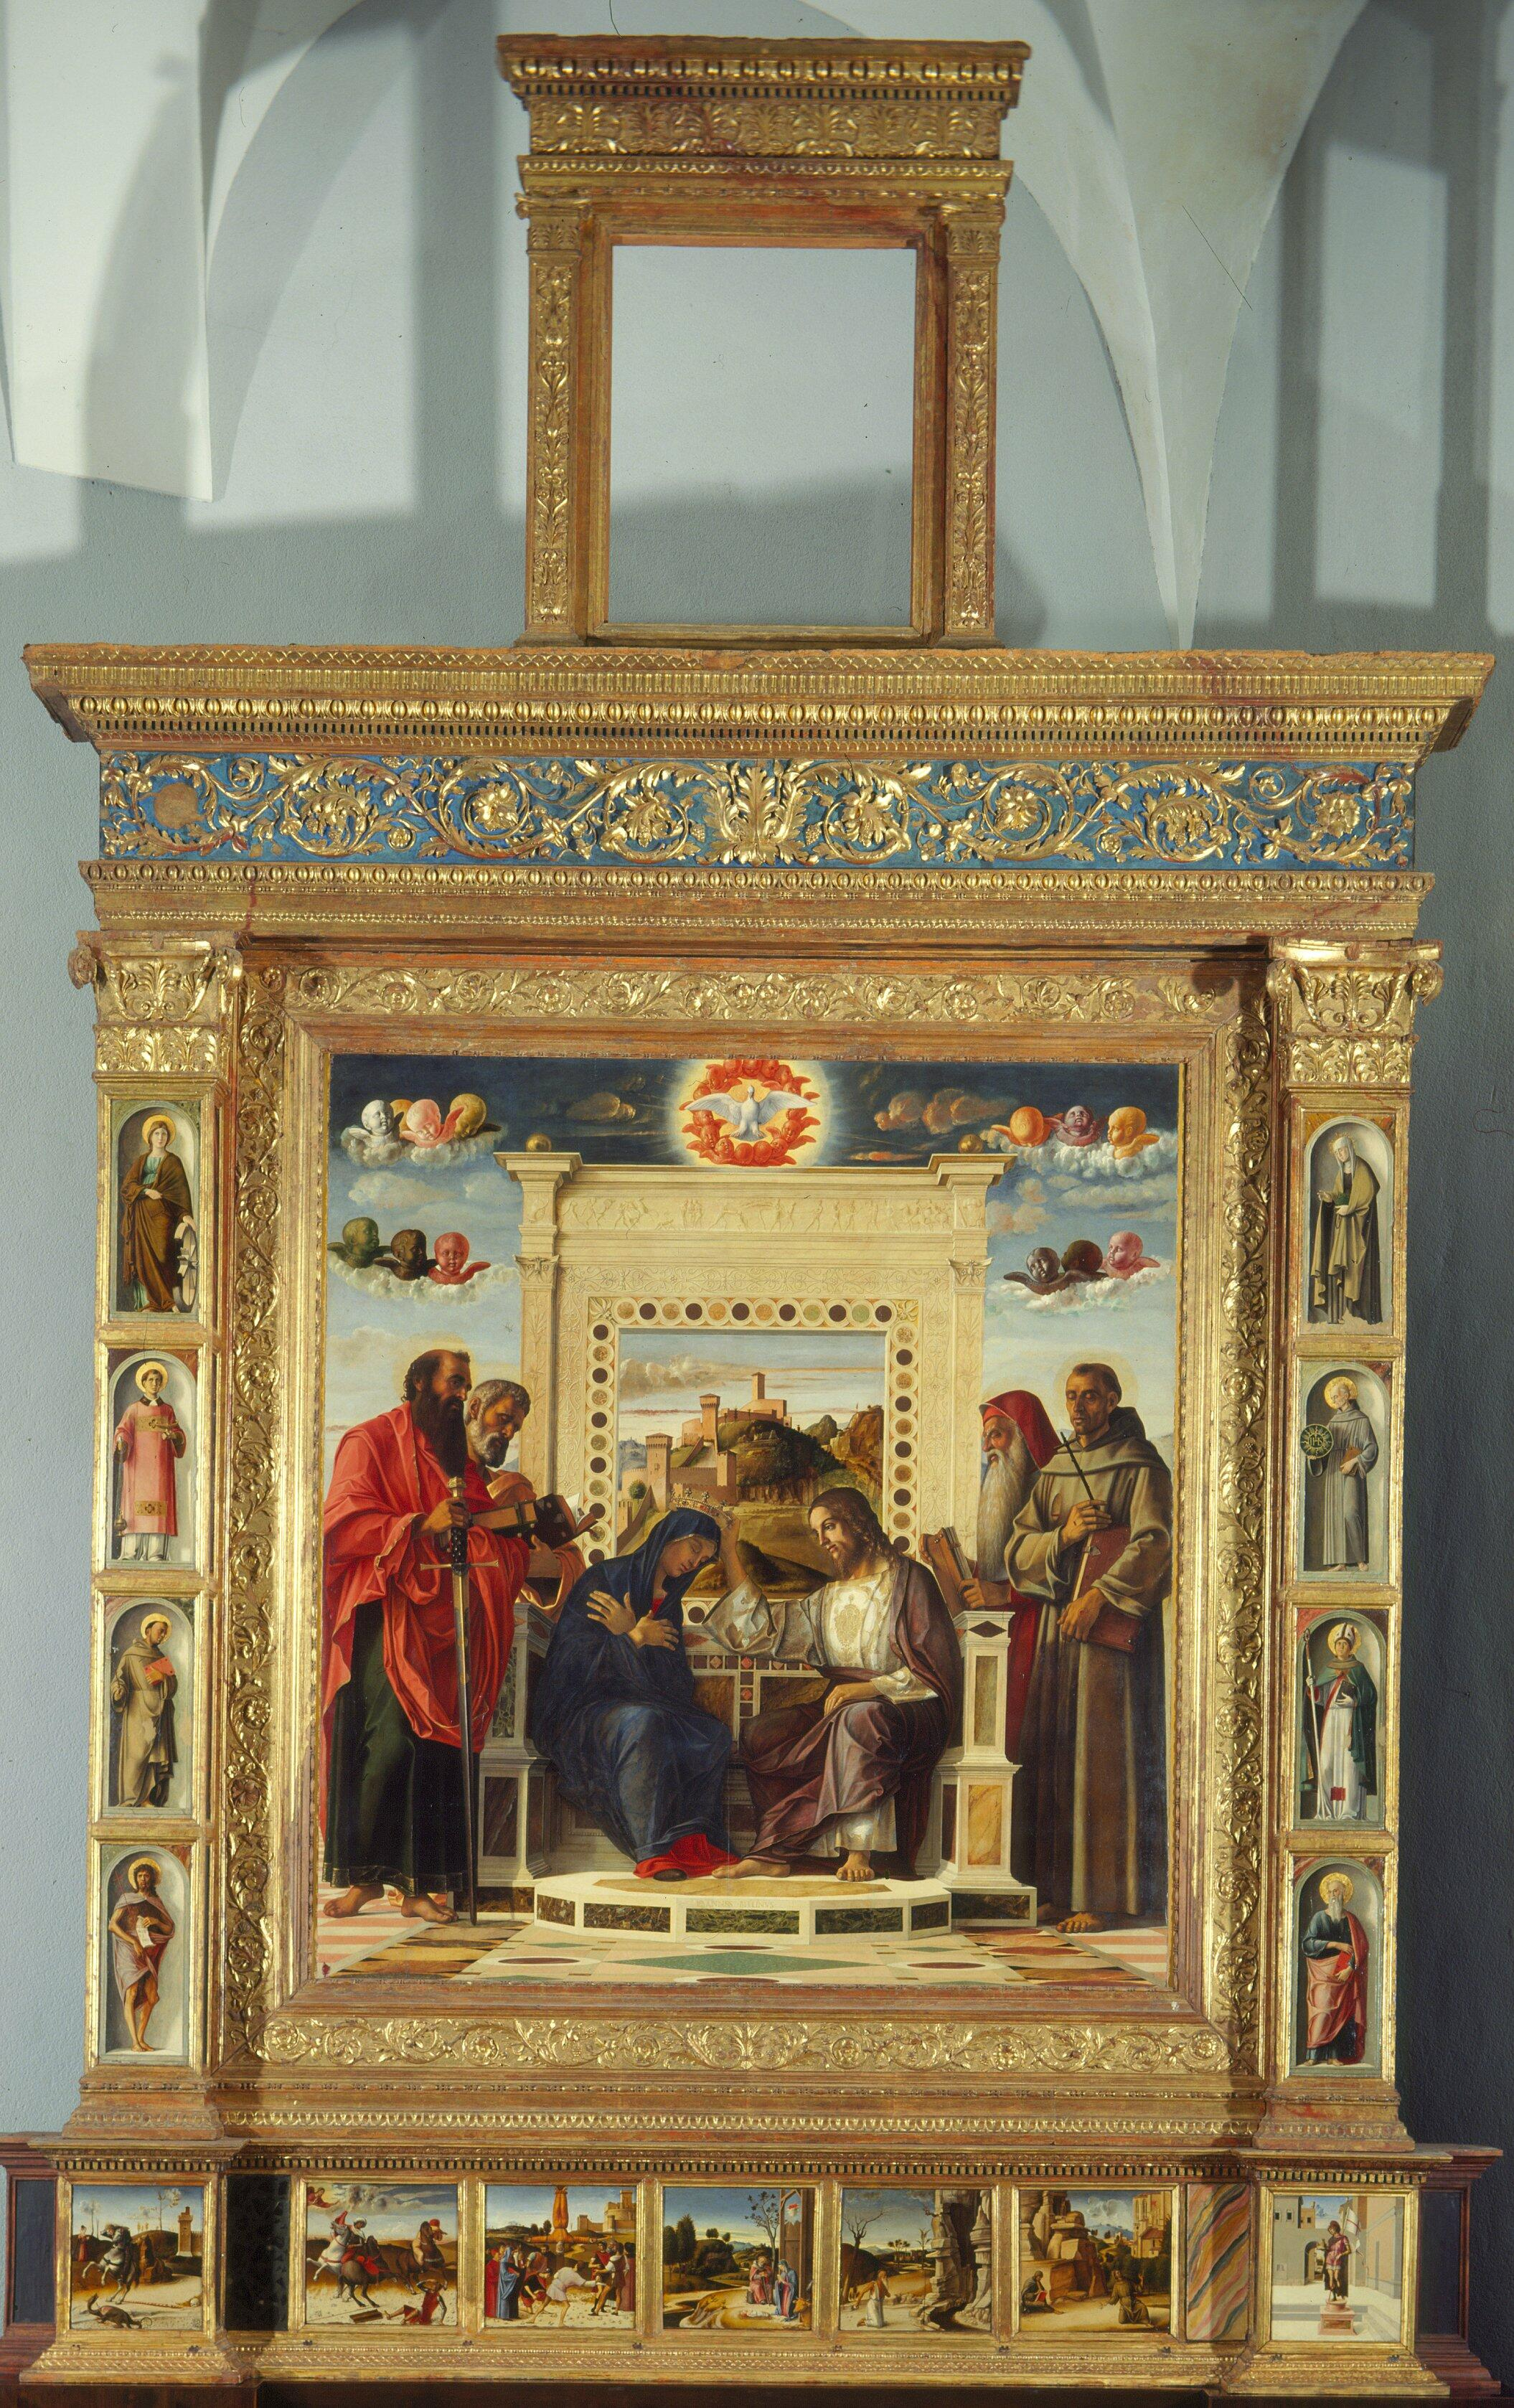
\includegraphics[scale=0.085]{Bellini_Giovanni-Incoronazione_della_Vergine.jpg}}
			\bigskip
			\newline
			\begin{minipage}{0.8\linewidth}
				\raggedright
				La pala, uno straordinario lavoro di carpenteria, costruito in vista, di un estrema semplicità di montaggio e tenuto insieme mirabilmente da pochi cavicchi di legno, fu dipinta per l'altare maggiore della chiesa di San Francesco a Pesaro.
			\end{minipage}
		}
	\end{tabularx}

	% Background image
	\AddToShipoutPictureBG*{\includegraphics[draft=false, width=\paperwidth,height=\paperheight]{example-image-plain}}
	\newpage
		
	%--------- Page 2 ----------
	
	% First line 
	\begin{tabularx}{\textwidth}{XX}
	{
		\hspace{12mm}
		%Vitale da Bologna - Sant'Ambrogio in trono
		\setdf{content={\textcolor{white}{\hspace{18mm} \Large \#3}}}
		\colorbox{black}{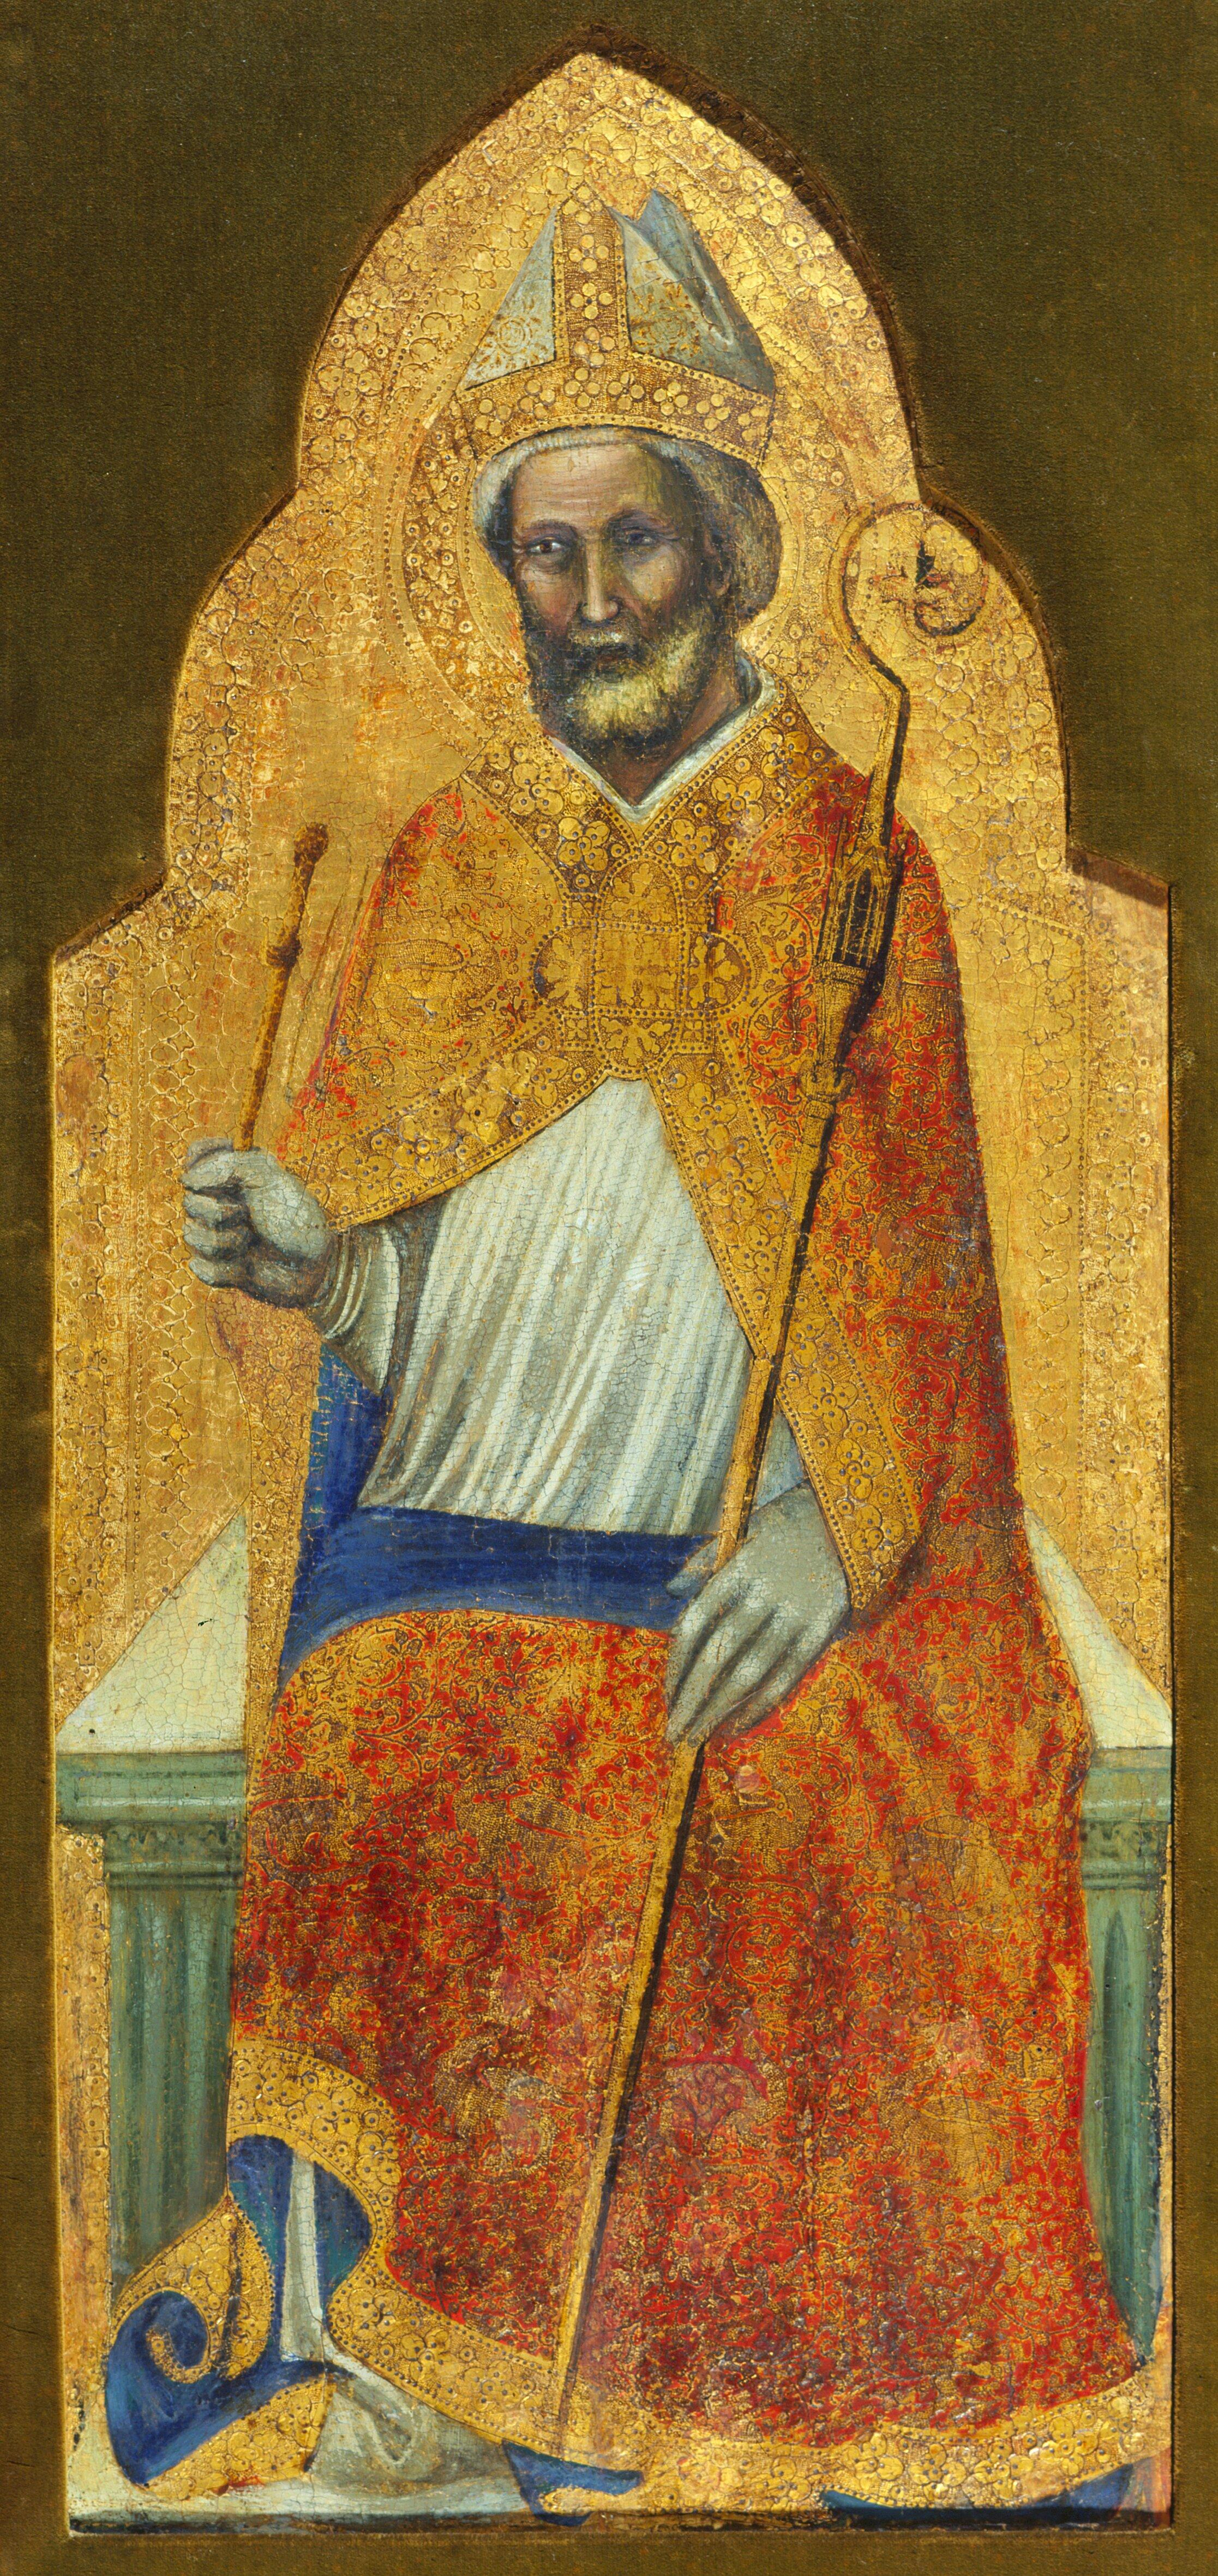
\includegraphics[scale=0.06]{Vitale_da_Bologna-Santo_Ambrogio_in_trono.jpg}}
		\bigskip
		\newline
		\begin{minipage}{0.8\linewidth}
			\raggedright
			Nonostante sia stata sottoposta in tempi recenti a restauro, la tavola presenta ancora nella superficie pittorica varie abrasioni, dovute forse ad antichi restauri, che ne compromettono in parte la leggibilità. Ciò è evidente soprattutto nella zona del viso del santo, fortemente consunta e priva ormai, nella resa dell'incarnato, di quelle connotazioni più morbidamente sfumate che sono tipiche dell'arte vitalesca.
			
		\end{minipage}
		
	}&{
			\hspace{1.5mm}
			% Desani Pietro - Rebecca ed Eleazar
			\setdf{content={\textcolor{white}{\hspace{35mm} \Large \#4}}}
			\colorbox{black}{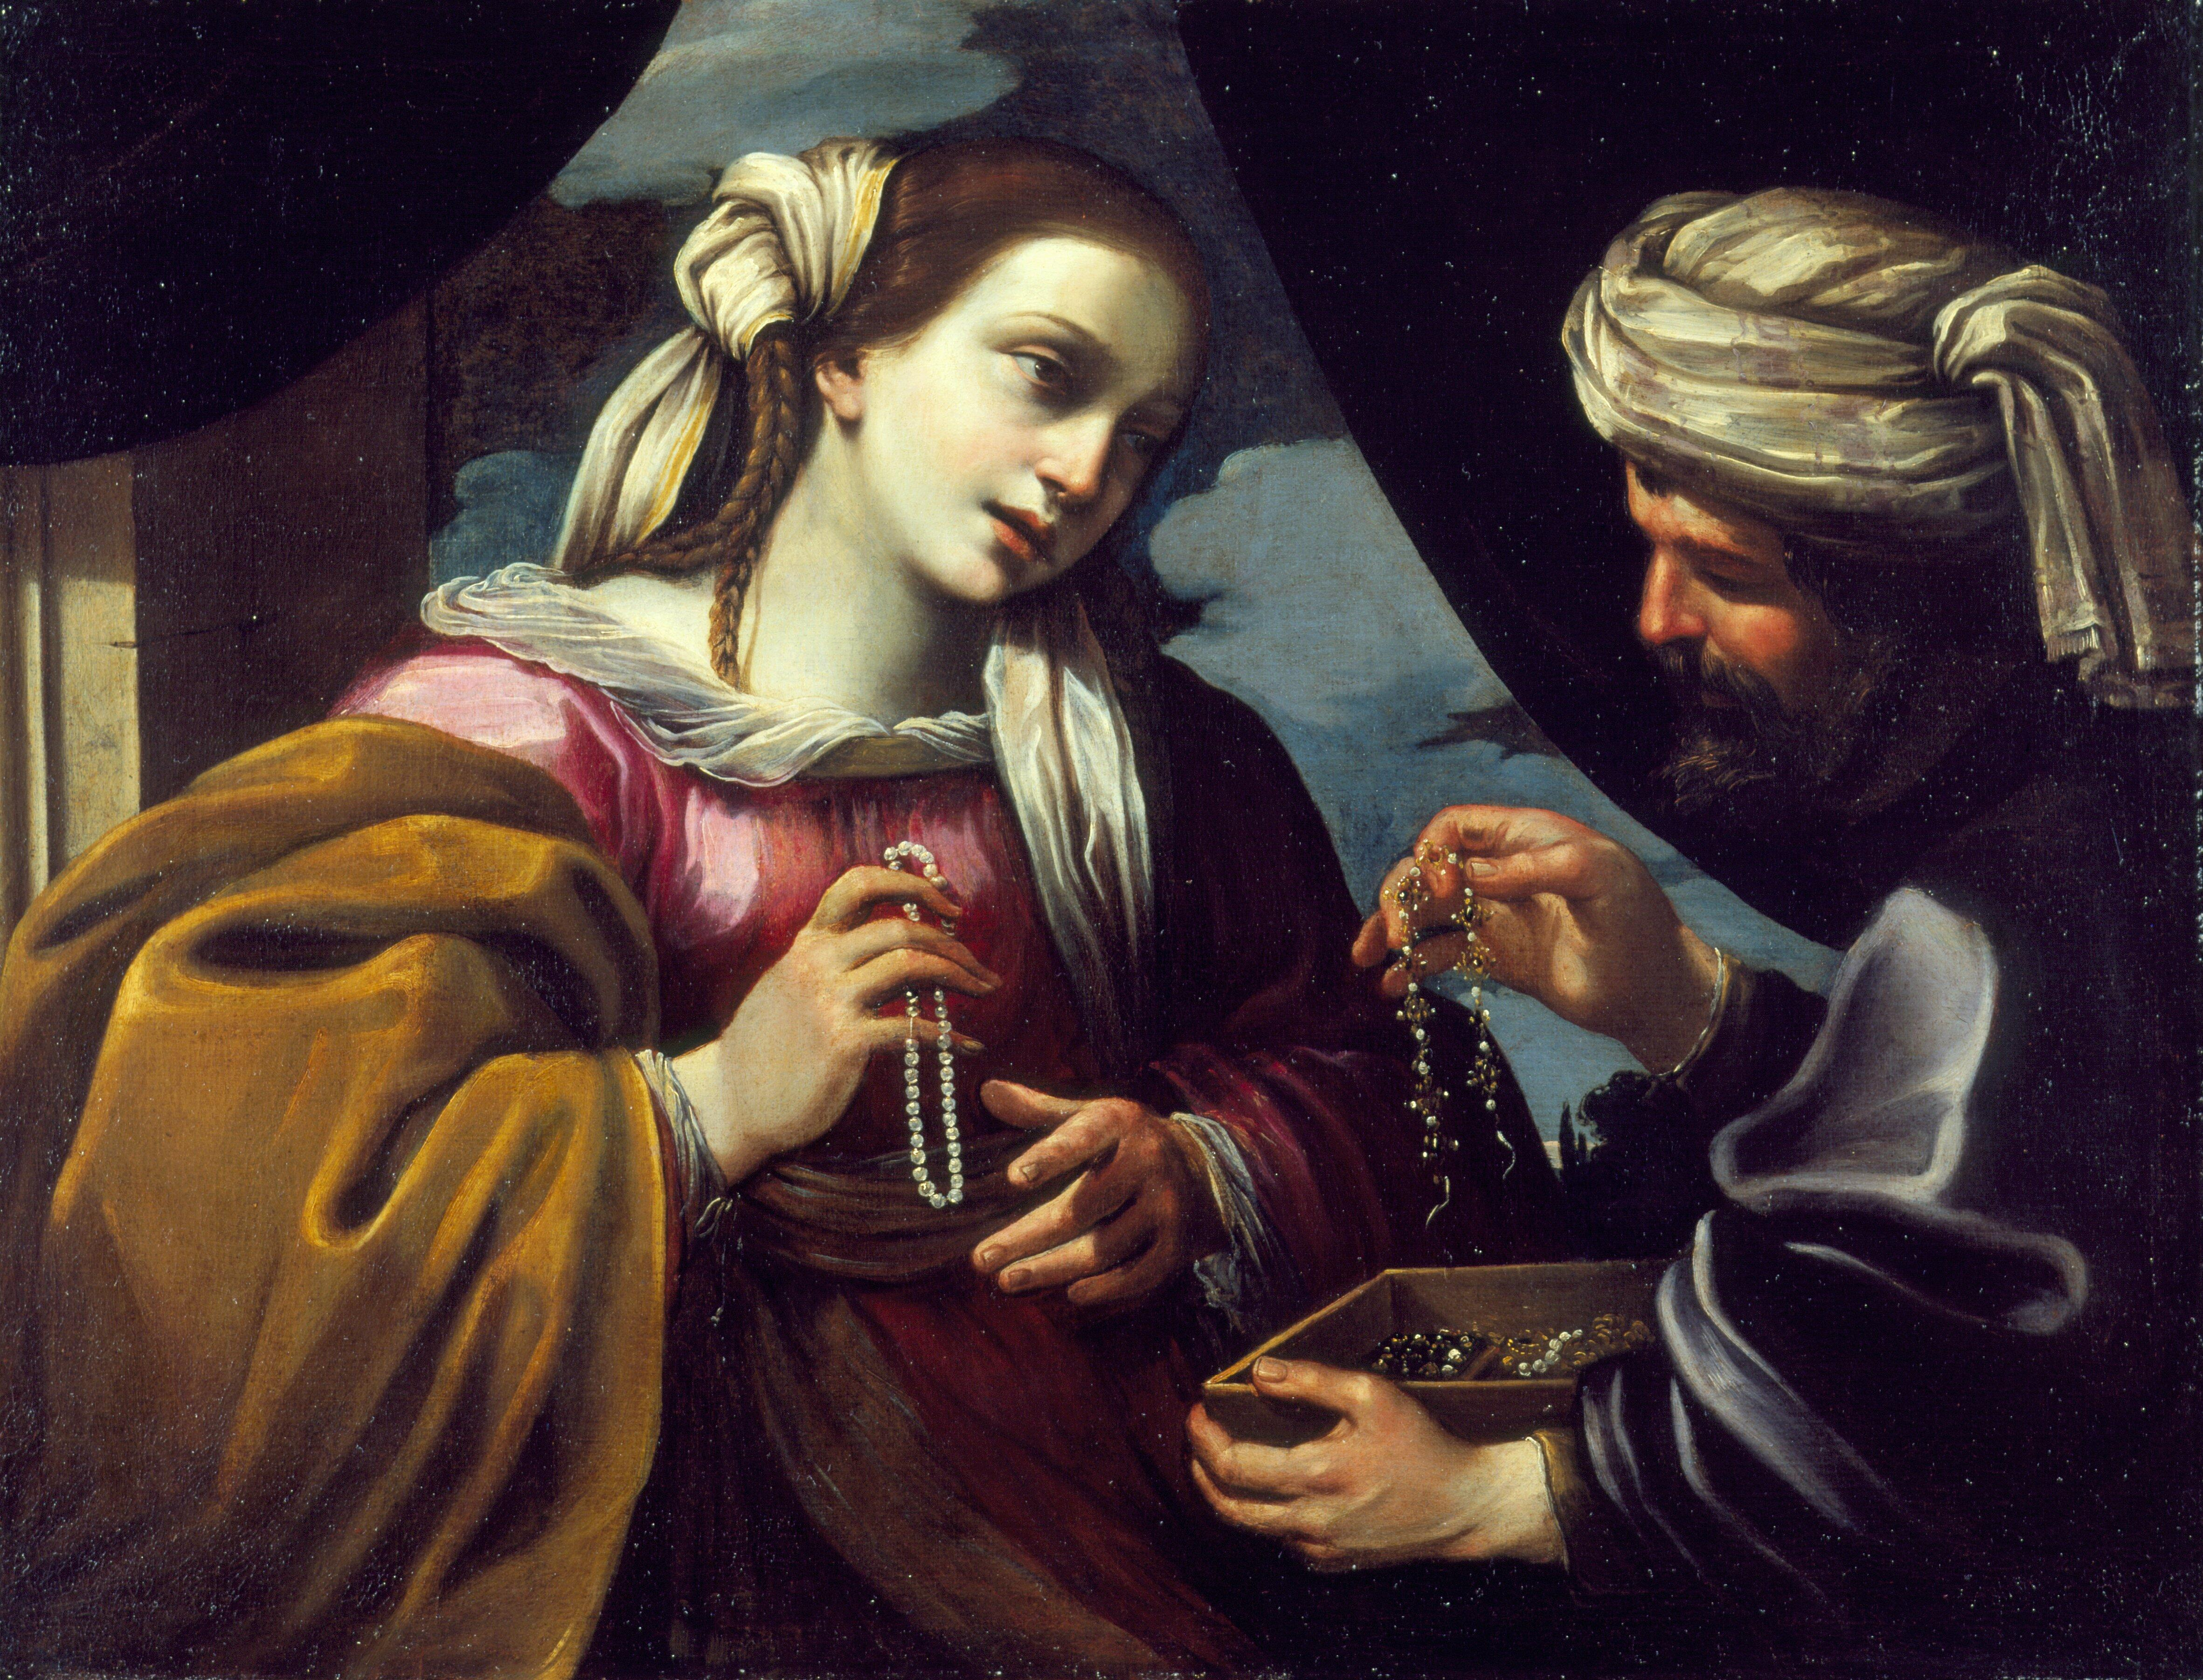
\includegraphics[scale = 0.05]{Desani_Pietro-Rebecca_ed_Eleazar.jpg}}
			\bigskip
			\newline
			\begin{minipage}{0.9\linewidth}
				\raggedright
				Il fido Eleazar, mandato in Mesopotamia da Abramo per cercare una sposa per suo figlio Isacco incontra a un pozzo una fanciulla che lo disseta e alla quale consegna i gioielli che gli sono stati dati per l'eletta.\\
				Secondo quanto si apprende dalle ricerche condotte in questa occasione da Barbara Ghelfi, il dipinto venne ereditato nel 1806 da Maria Malvezzi: nell'occasione veniva detto "Due mezze figure che contrattano delle gioie, d´uno stile che somiglia il Tiarini".
			\end{minipage} 
		}
	\end{tabularx}

	% Second line
	\nopagebreak
	\begin{tabularx}{\textwidth}{X}
	{	
		\begin{center}
			\hspace{27mm}
			%Giovanni Antonio Garella - Leda e il cigno
			\setdf{content={\textcolor{white}{\hspace{20mm} \Large \#5}}}
			\colorbox{black}{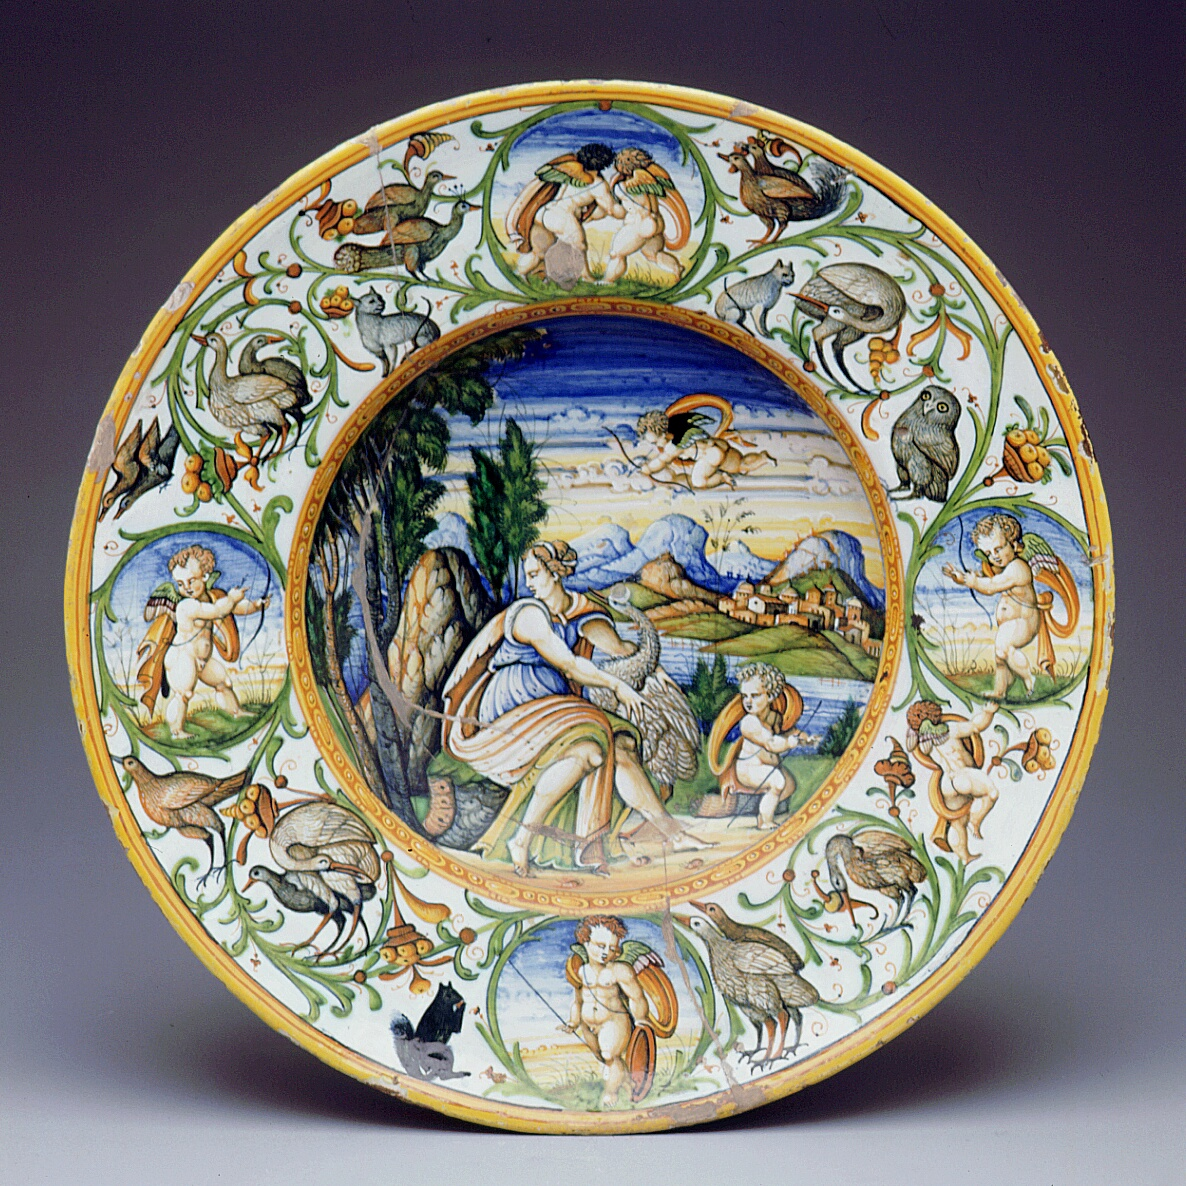
\includegraphics[]{Giovanni_Antonio_Garella-Leda_e_il_cigno.jpg}}
			\bigskip
			\newline
			\begin{minipage}{0.9\linewidth}
					\raggedright
					Il pezzo va riferito senza dubbio alcuno al "Maestro della Conversione di San Paolo": appartengono alla sua mano i caratteri del paesaggio e delle figure, come per esempio il profilo di Leda, che richiama con puntualità quelli degli dipinti sulla tesa.\\
					Ci troviamo di fronte ad un maestro particolarmente capace sia nell'esecuzione delle scene istoriate, sia nella creazione delle raffaellesche, queste ultime eseguite con grande inventiva di dettagli e con mano sicura, molto distanti anche nella tipologia da quelle dei Fontana oppure dei Patanazzi.
			\end{minipage}
		\end{center}
	}
	\end{tabularx}
	
	% Background image
	\AddToShipoutPictureBG*{\includegraphics[draft=false, width=\paperwidth,height=\paperheight]{example-image-plain}}
	\newpage
	
	%--------- Page 3 ----------
	
	% First line 
	\vspace*{-10mm}
	%\vspace*{\fill}
	\begin{tabularx}{\textwidth}{XX}
		{
			\begin{center}
				\hspace{5mm}
				%Specchio in vetro di Murano
				\setdf{content={\textcolor{white}{\hspace{25mm} \Large \#6}}}
				\colorbox{black}{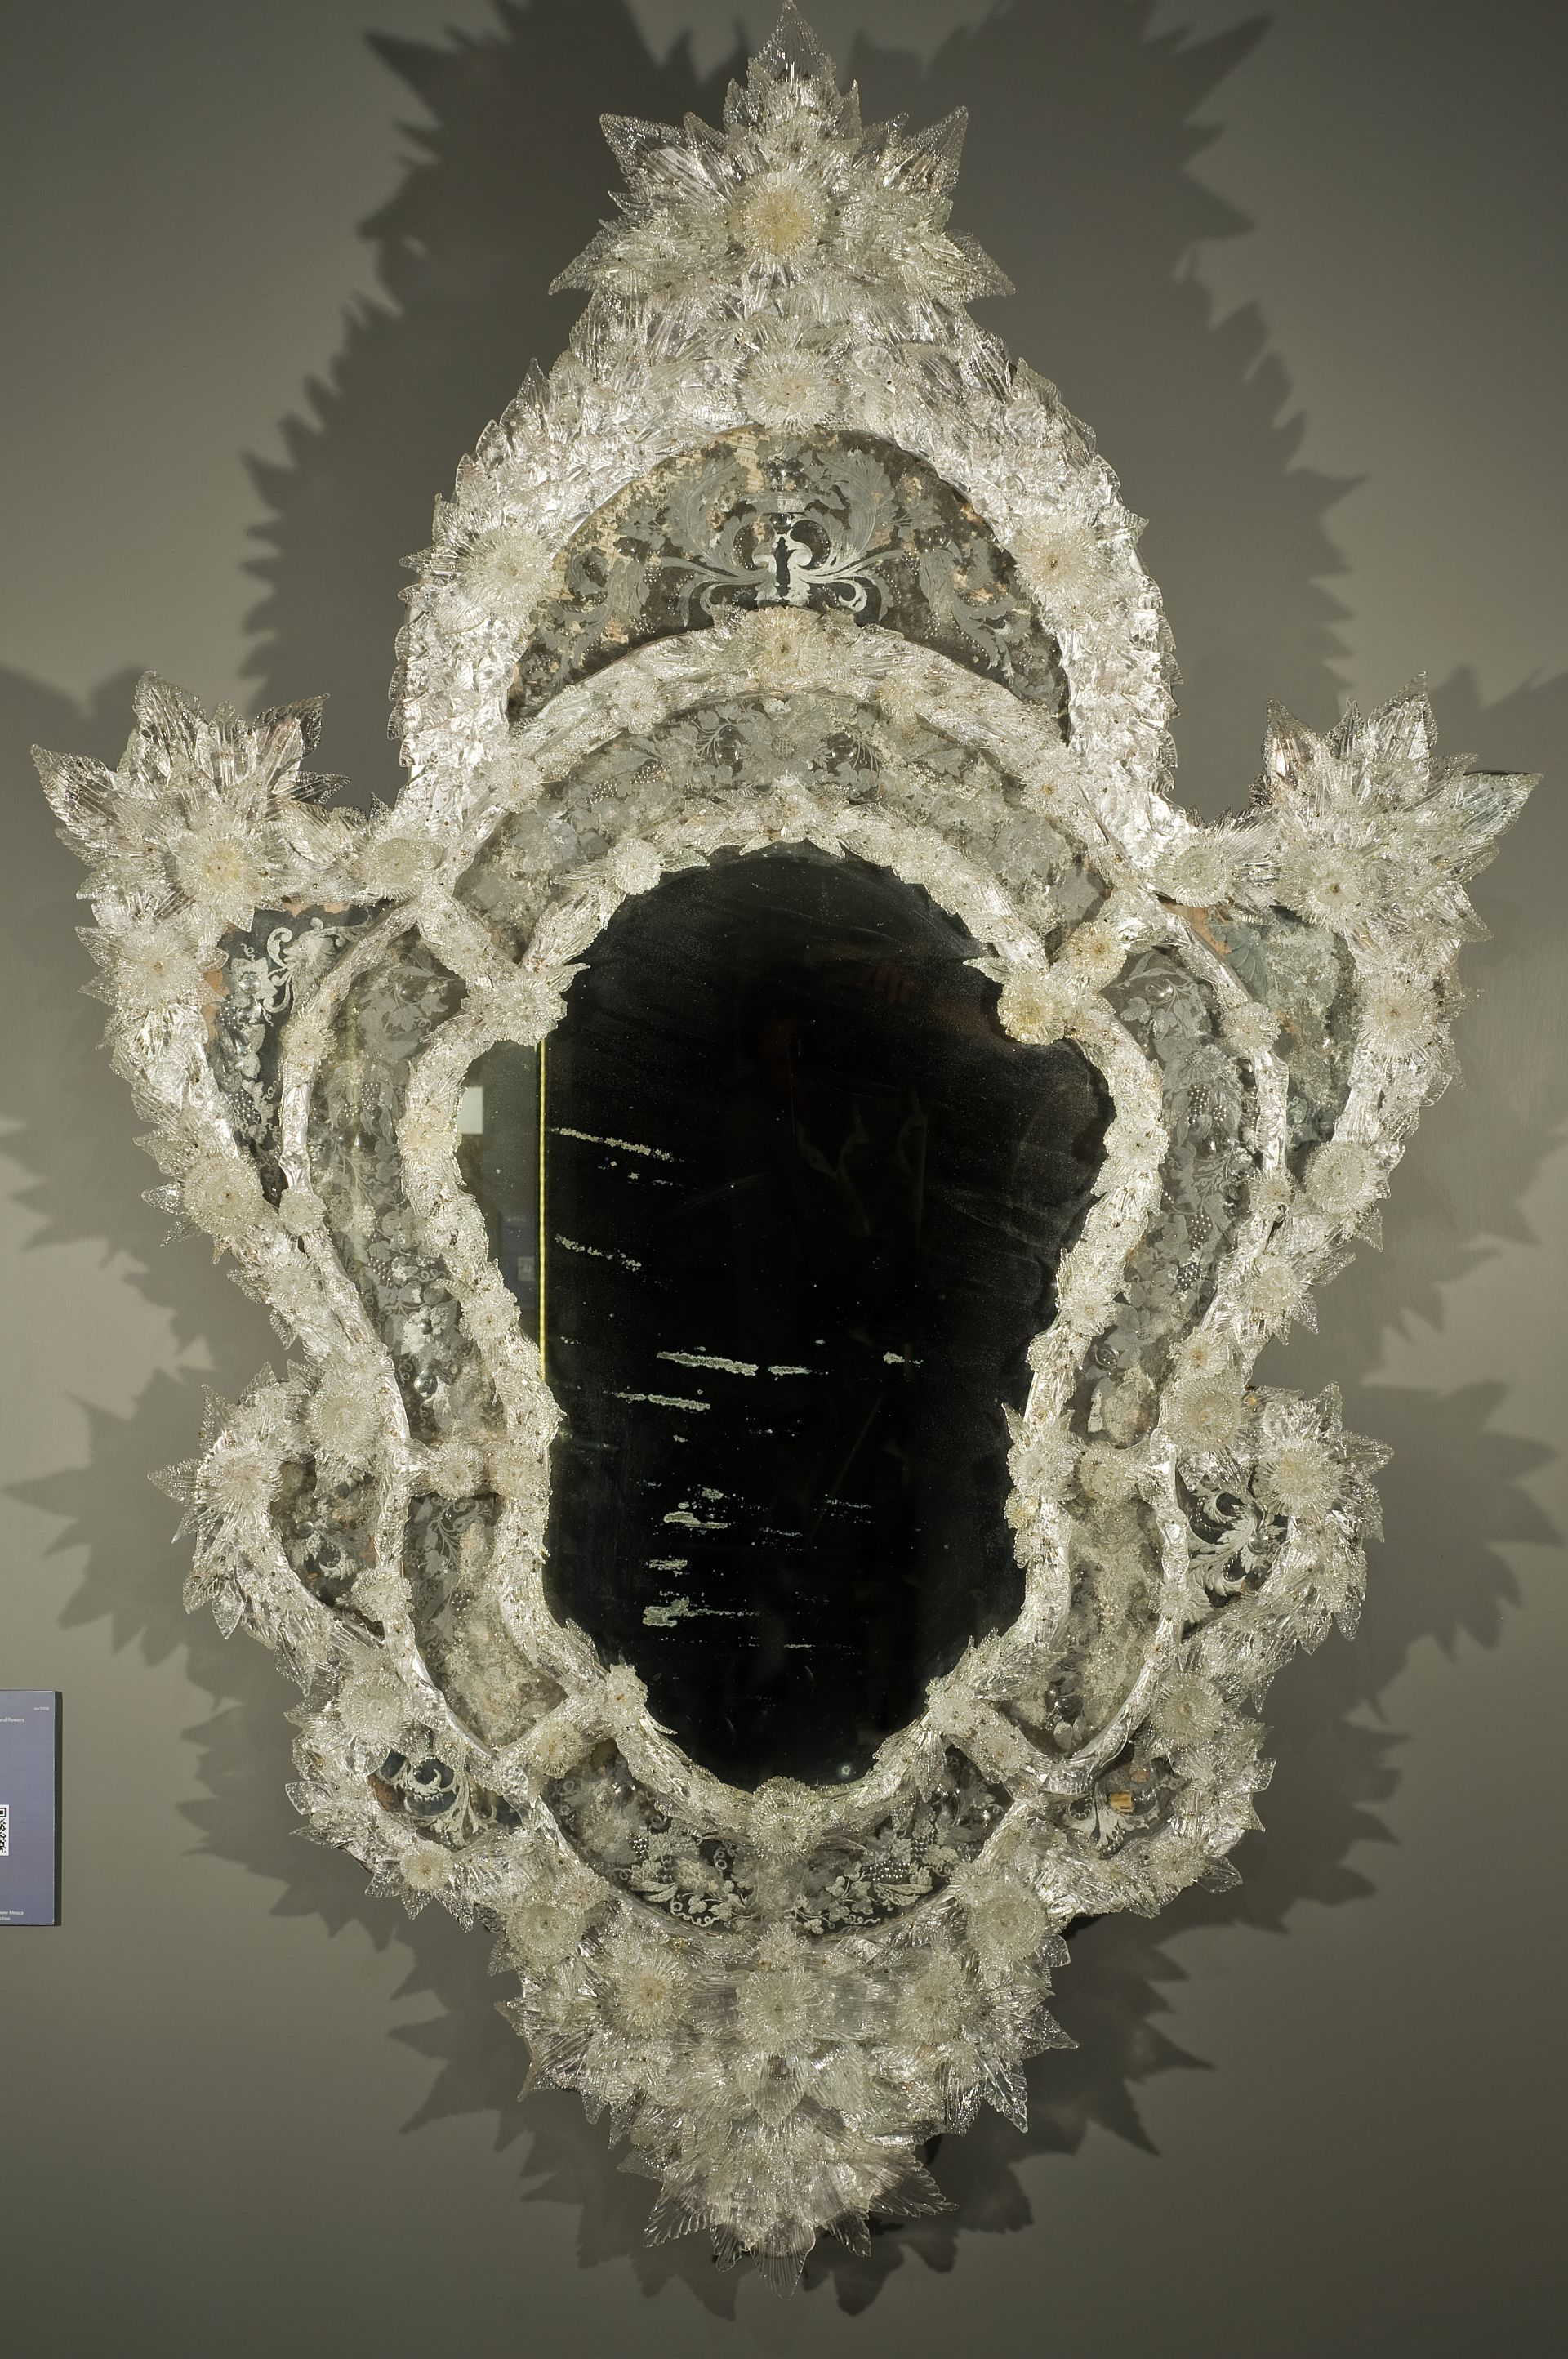
\includegraphics[scale=0.3]{Specchio_di_Murano.jpg}}
				\bigskip
				\newline
				\begin{minipage}{0.8\linewidth}
					\raggedright
					L'opera è una specchiera, si definiscono infatti così gli specchi con cornice fatti per essere appesi alle pareti a scopi funzionali e decorativi.\\ 
					Realizzata tra la fine del Settecento e l'inizio dell'Ottocento, è decorata con foglie e fiori in vetro che costituiscono la  peculiarità delle specchiere artistiche di Murano.\\
					La produzione muranese nel Settecento eleva il livello medio della produzione ad un grado di eleganza e raffinatezza mai raggiunto prima.
				\end{minipage}
			\end{center}
			
		}&{
			\vspace{20mm}
				%Vedute di Roma
				\hspace{10mm}{
				\setdf{content={\textcolor{white}{\hspace{30mm} \Large \#7}}}
				\colorbox{black}{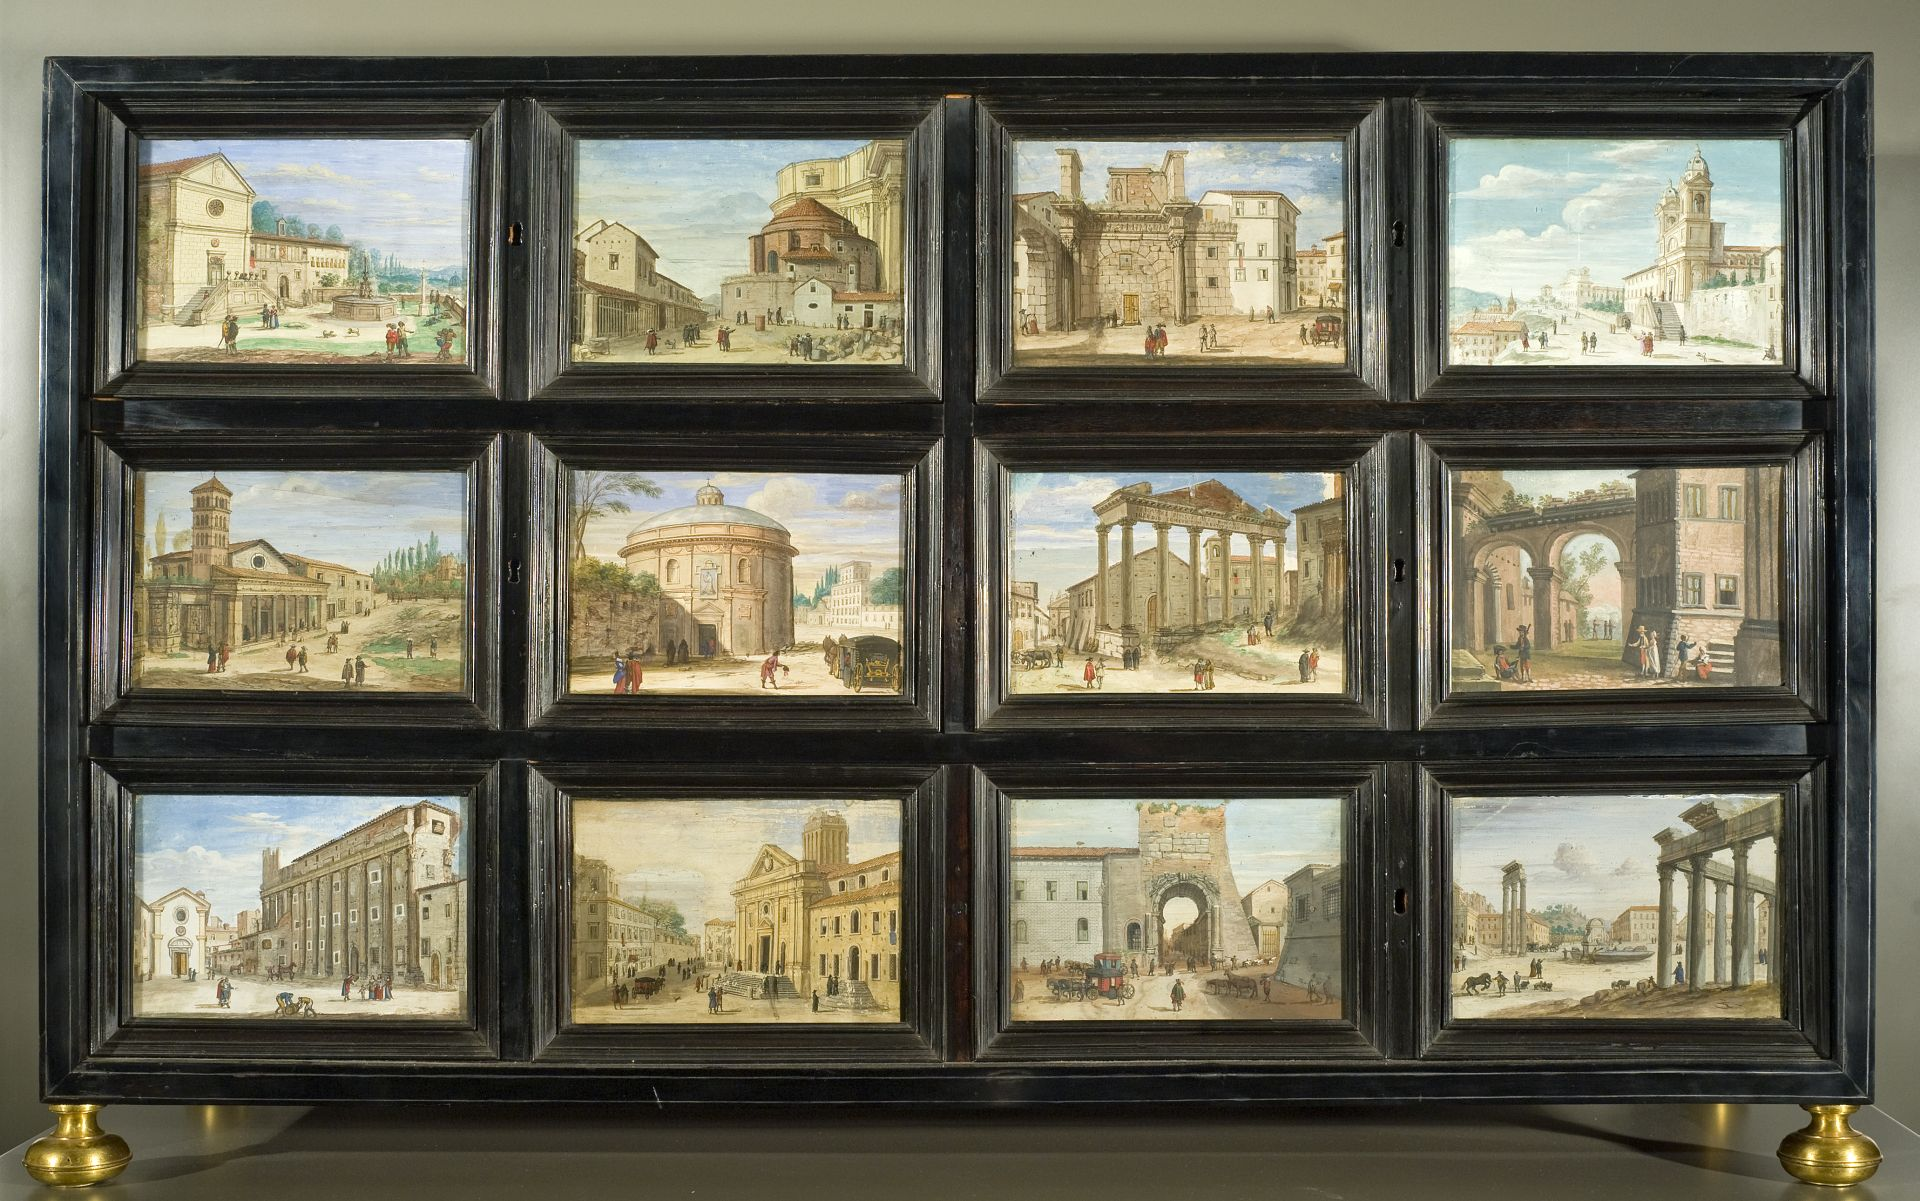
\includegraphics[scale=0.35]{Vedute_di_Roma_1.jpg}}
				}
				%\bigskip
				%\newline
				\begin{center}
					\begin{minipage}{0.7\linewidth}
						\raggedright
						L'usanza di decorare il fronte di stipi e studioli con placche raffiguranti vedute dell'urbe deve essere fatta risalire agli anni Sessanta del Seicento, come si può vedere nella parte interna dello stipo eseguito dall'ebanista Giacomo Herman nel 1668 e attualmente al Kunsthistorisches Museum di Vienna. Va inoltre notato che il tipo di veduta che tende a riprodurre in maniera pressoché fedele il luogo rappresentato si afferma a Roma attorno agli anni Trenta del Seicento, con la presenza a Roma del pittore strasburghese Willhelm Baur.
					\end{minipage}
				\end{center}
		}
	\end{tabularx}
	%\vspace*{\fill}
	
	% Second line
	\nopagebreak
	\begin{tabularx}{\linewidth}{XX}
		{}&{
			\hspace{15mm}
			\setdf{content={\textcolor{white}{\hspace{20mm} \Large \#8}}}
			\colorbox{black}{\includegraphics[scale=0.2]{Orologio_notturno.jpg}}
			\bigskip
			\newline
			\begin{minipage}{0.9\linewidth}
				\raggedright
				Cassa non pertinente all'orologio, assemblata nel XIX secolo con una secentesca scultura barocca di legno dorato.
				Sulla mostra in rame sono dipinte le quattro stagioni su cui l'allegoria del tempo passa veloce ad ali spiegate.
			\end{minipage}
		}
	\end{tabularx}
	
	% Background image
	\AddToShipoutPictureBG*{\includegraphics[draft=false, width=\paperwidth,height=\paperheight]{example-image-plain}}
	\newpage
	
	%--------- Page 4 ----------
	
	% First line
		\hspace{5mm}{
	\begin{tabularx}{\linewidth}{XX}
		{		
				\hspace{5mm}
				%Milani Aureliano - Mercato
				\setdf{content={\textcolor{white}{\hspace{25mm} \Large \#9}}}
				\colorbox{black}{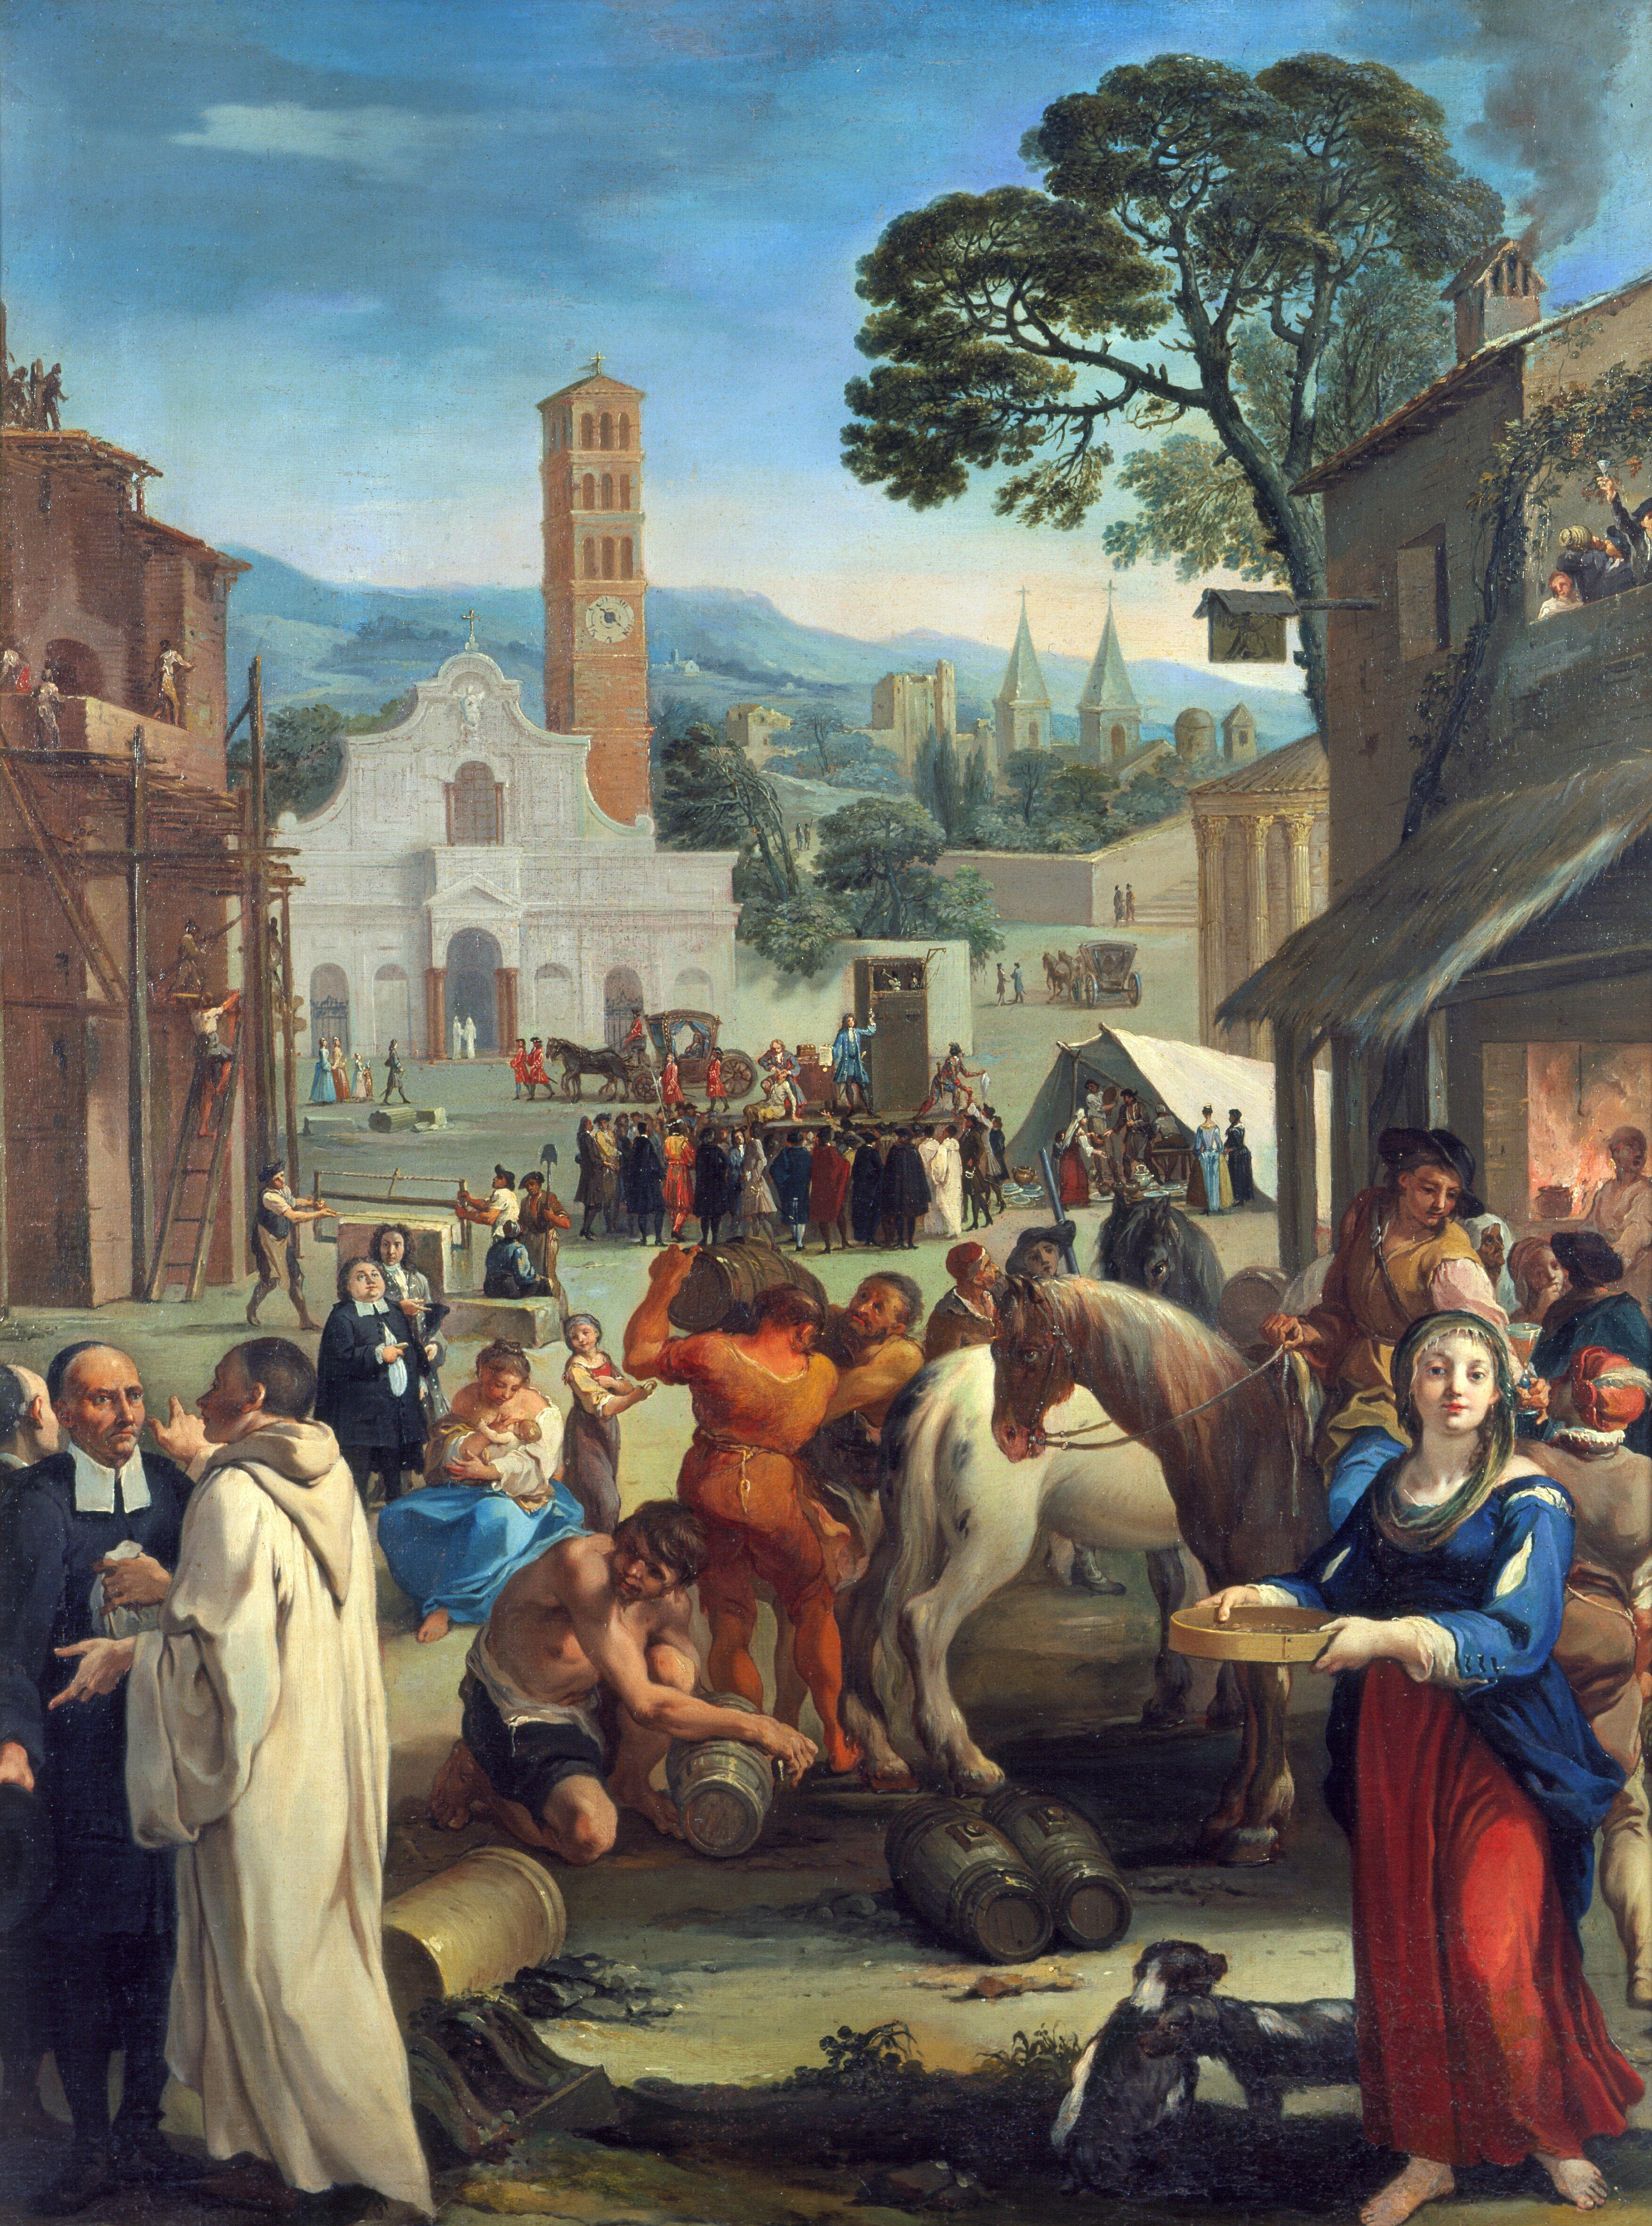
\includegraphics[scale=0.05]{Milani_Aureliano-Mercato.jpg}}
				\bigskip
				\newline
				\begin{minipage}{0.8\linewidth}
					\raggedright
					La chiesa nel fondo è stata riconosciuta in Santa Maria in Cosmedin a Roma, la cui facciata venne ultimata nel 1718 su disegno di Giuseppe Sardi. La denominazione della piazza antistante deriva dalla presenza di un mascherone romano sotto il portico, noto tra il popolino come "bocca della Verità".
				\end{minipage}
		}&{
				\hspace{3mm}
				%Berentz Christian - Fiori e frutta con bicchieri di cristallo
				\setdf{content={\textcolor{white}{\hspace{25mm} \Large \#10}}}
				\colorbox{black}{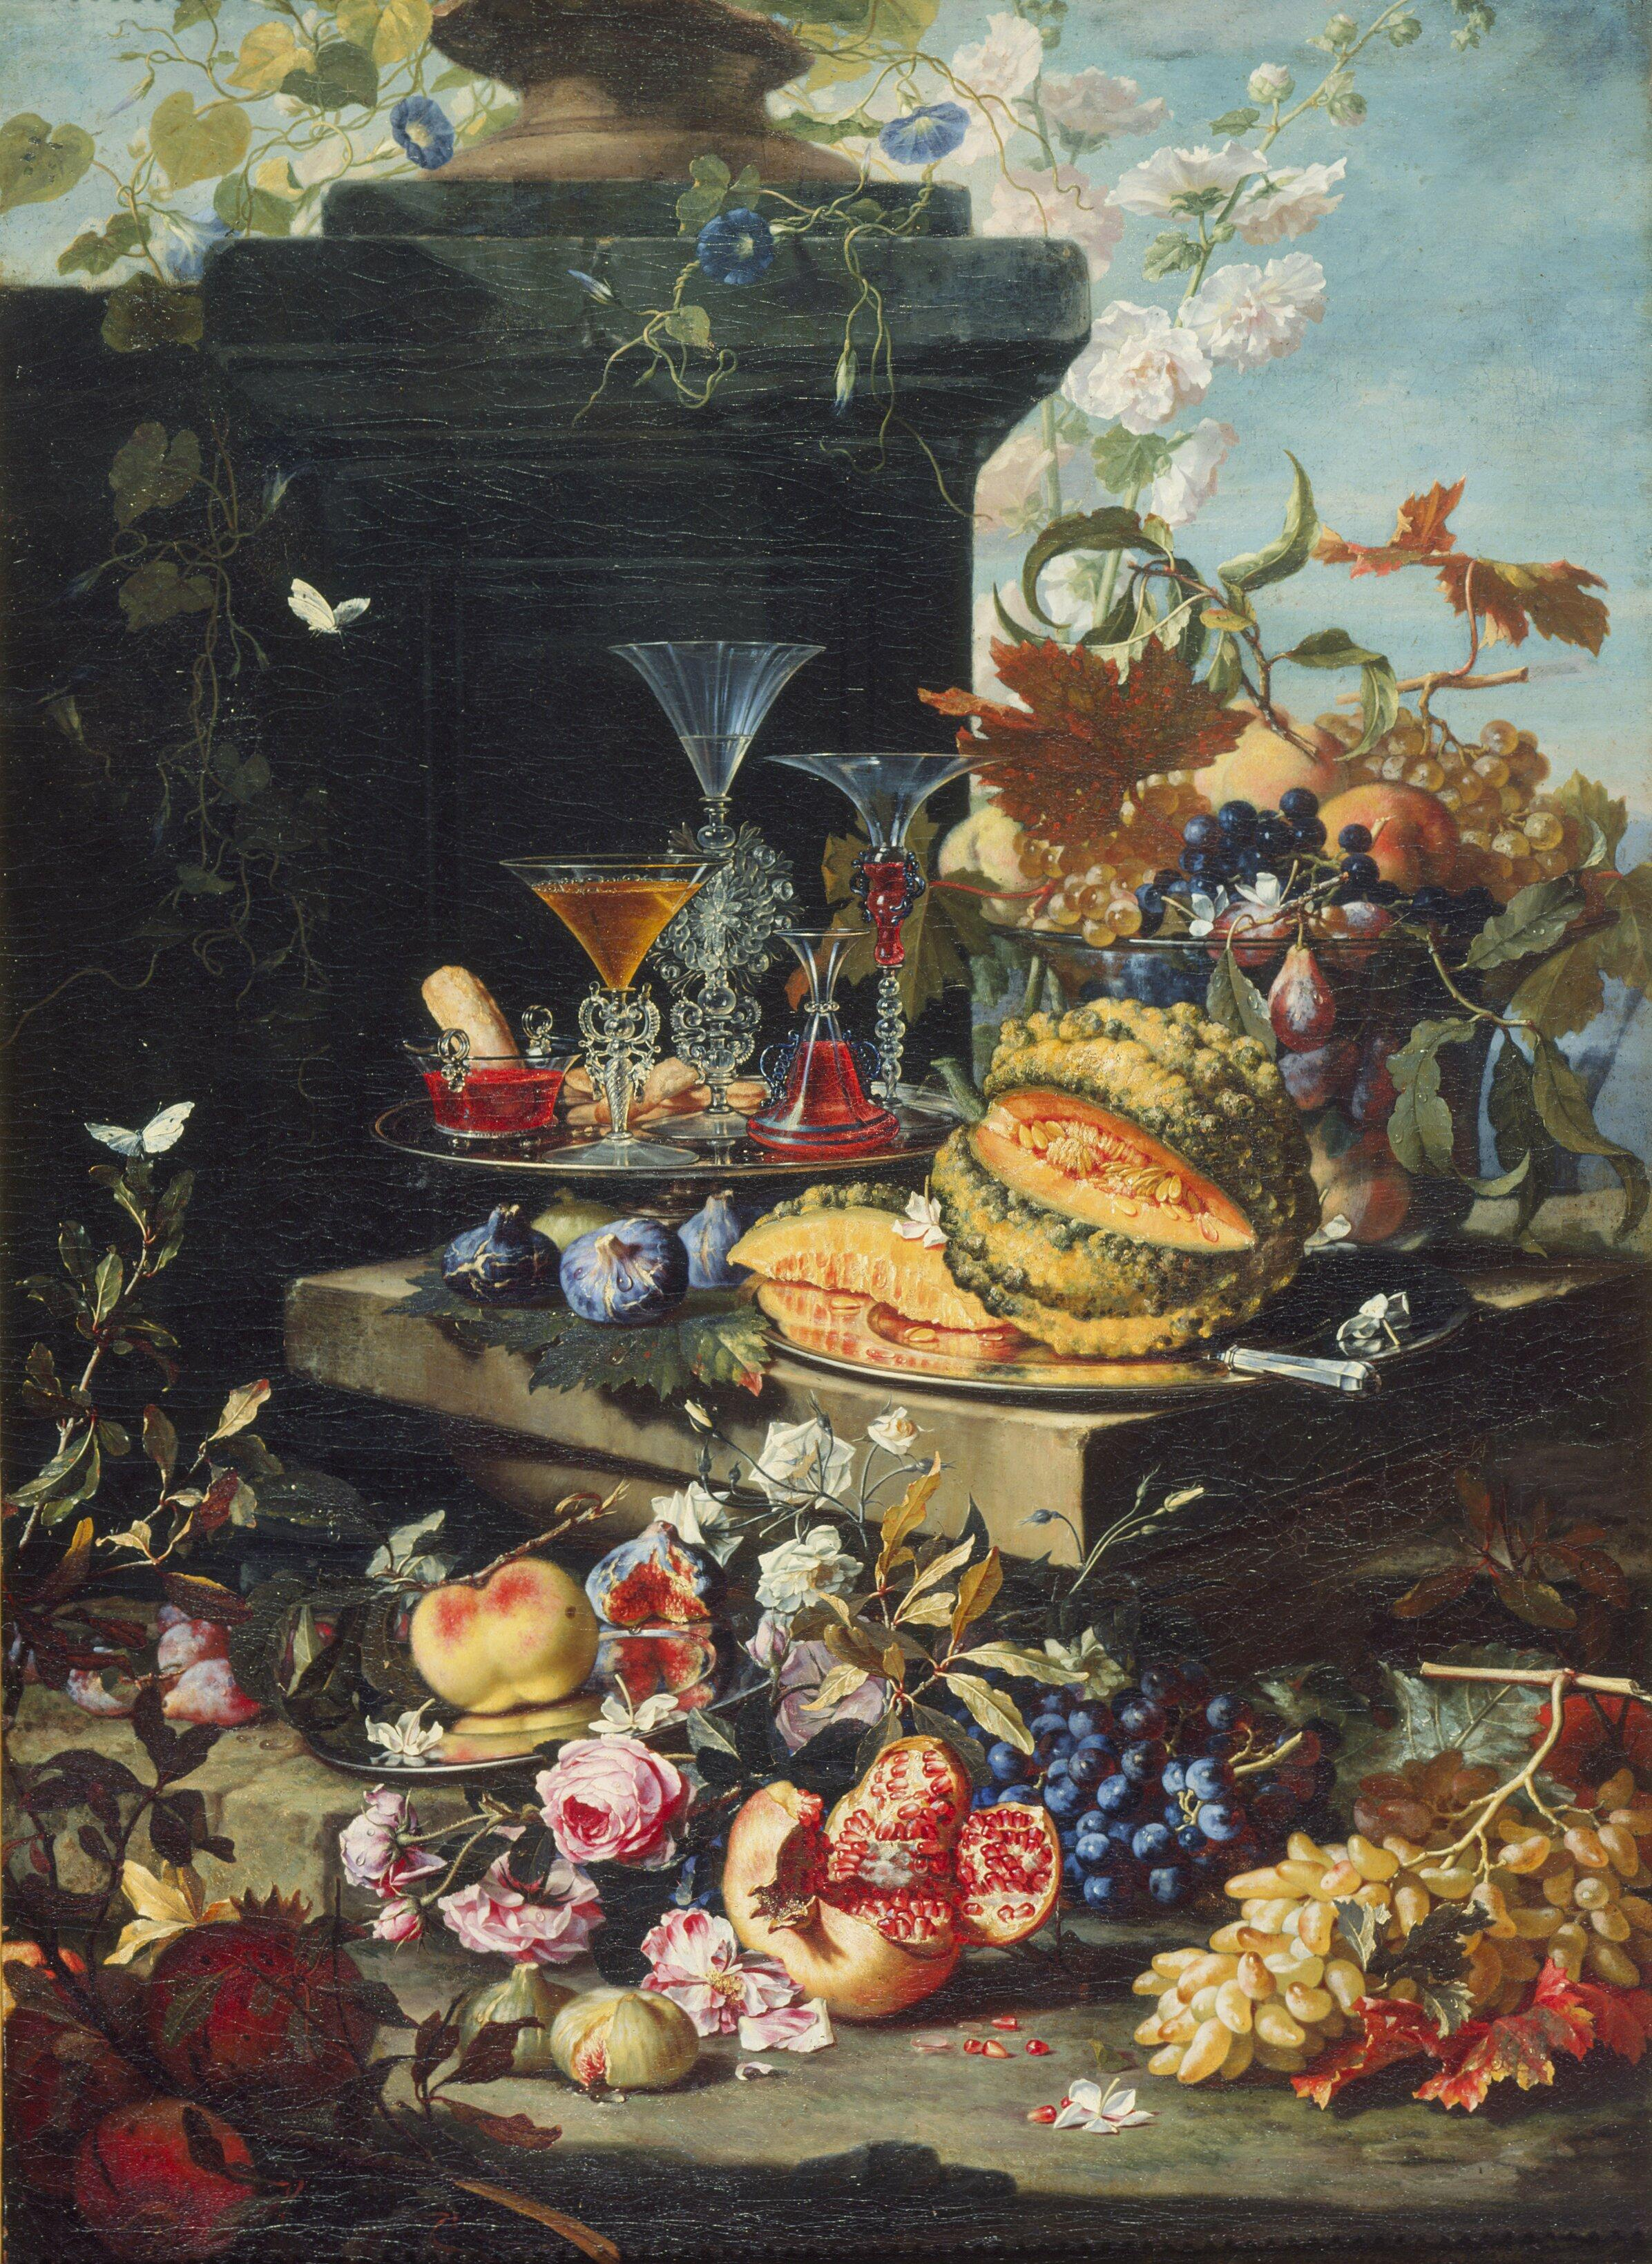
\includegraphics[scale= 0.08]{Berentz_Christian-Fiori_e_frutta_con_bicchieri_di_cristallo.jpg}}
				\bigskip
				\newline
				\begin{minipage}{0.8\linewidth}
					\raggedright
					Vero e proprio saggio di bravura del pittore amburghese giunto a Roma attorno al 1685, il dipinto coniuga la verità 'ottica' della cultura nordica con la teatralità della natura morta barocca romana.
				\end{minipage}
		}
	\end{tabularx}
	}

	% Second line
	\vspace{5mm}
	\hspace{5mm}{
	\nopagebreak
	\begin{tabularx}{\linewidth}{XX}
		{	
			\hspace{5mm}	
			%Gianlisi Antonio Junior - Trompe l'oeil con sonetto in onore di Eugenio di Savoia e mensola con oggetti
			\setdf{content={\textcolor{white}{\hspace{23mm} \Large \#11}}}
			\colorbox{black}{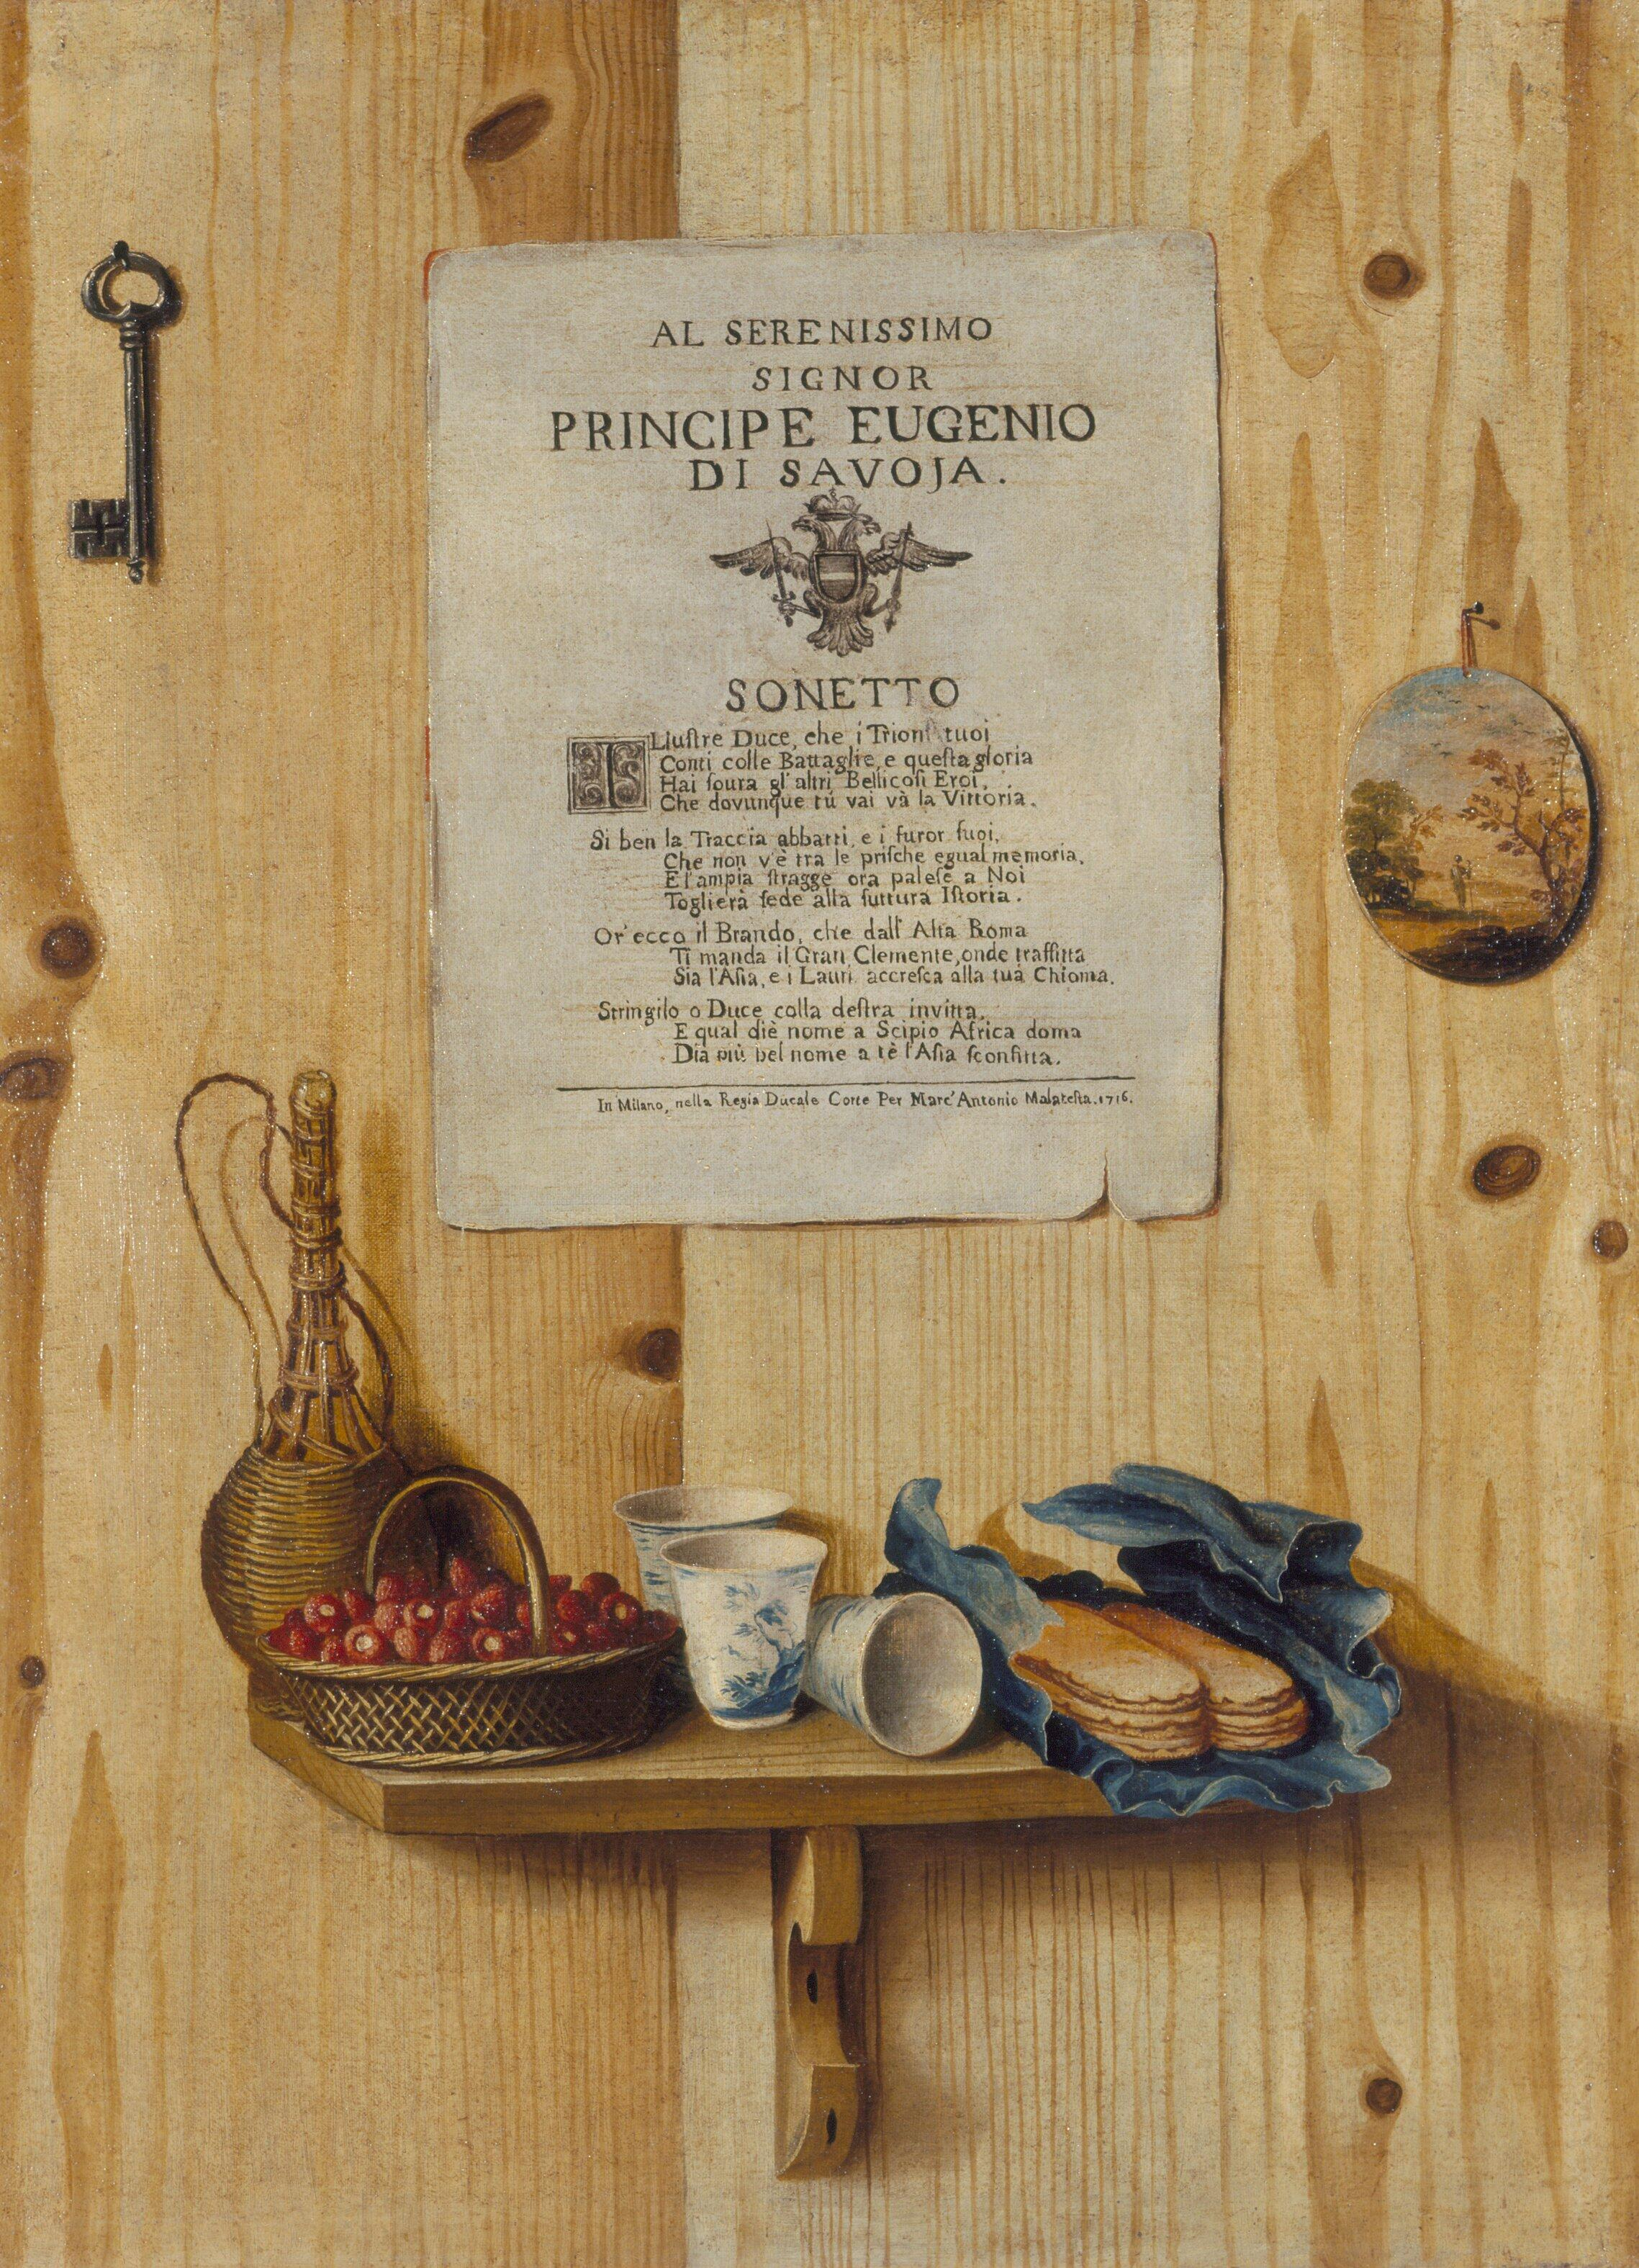
\includegraphics[scale=0.08]{Gianlisi_Antonio_Junior-Trompe_l_oeil_con_sonetto_in_onore_di_Eugenio_di_Savoia_e_mensola_con_oggetti.jpg}}
			\bigskip
			\newline
			\begin{minipage}{0.8\linewidth}
				\centering
				Informazioni~Mancanti.
			\end{minipage}
		}&{
			\hspace{5mm}
			%Gianlisi Antonio Junior - Trompe l'oeil con paesaggio forbici e mensola con oggetti
			\setdf{content={\textcolor{white}{\hspace{25mm} \Large \#12}}}
			\colorbox{black}{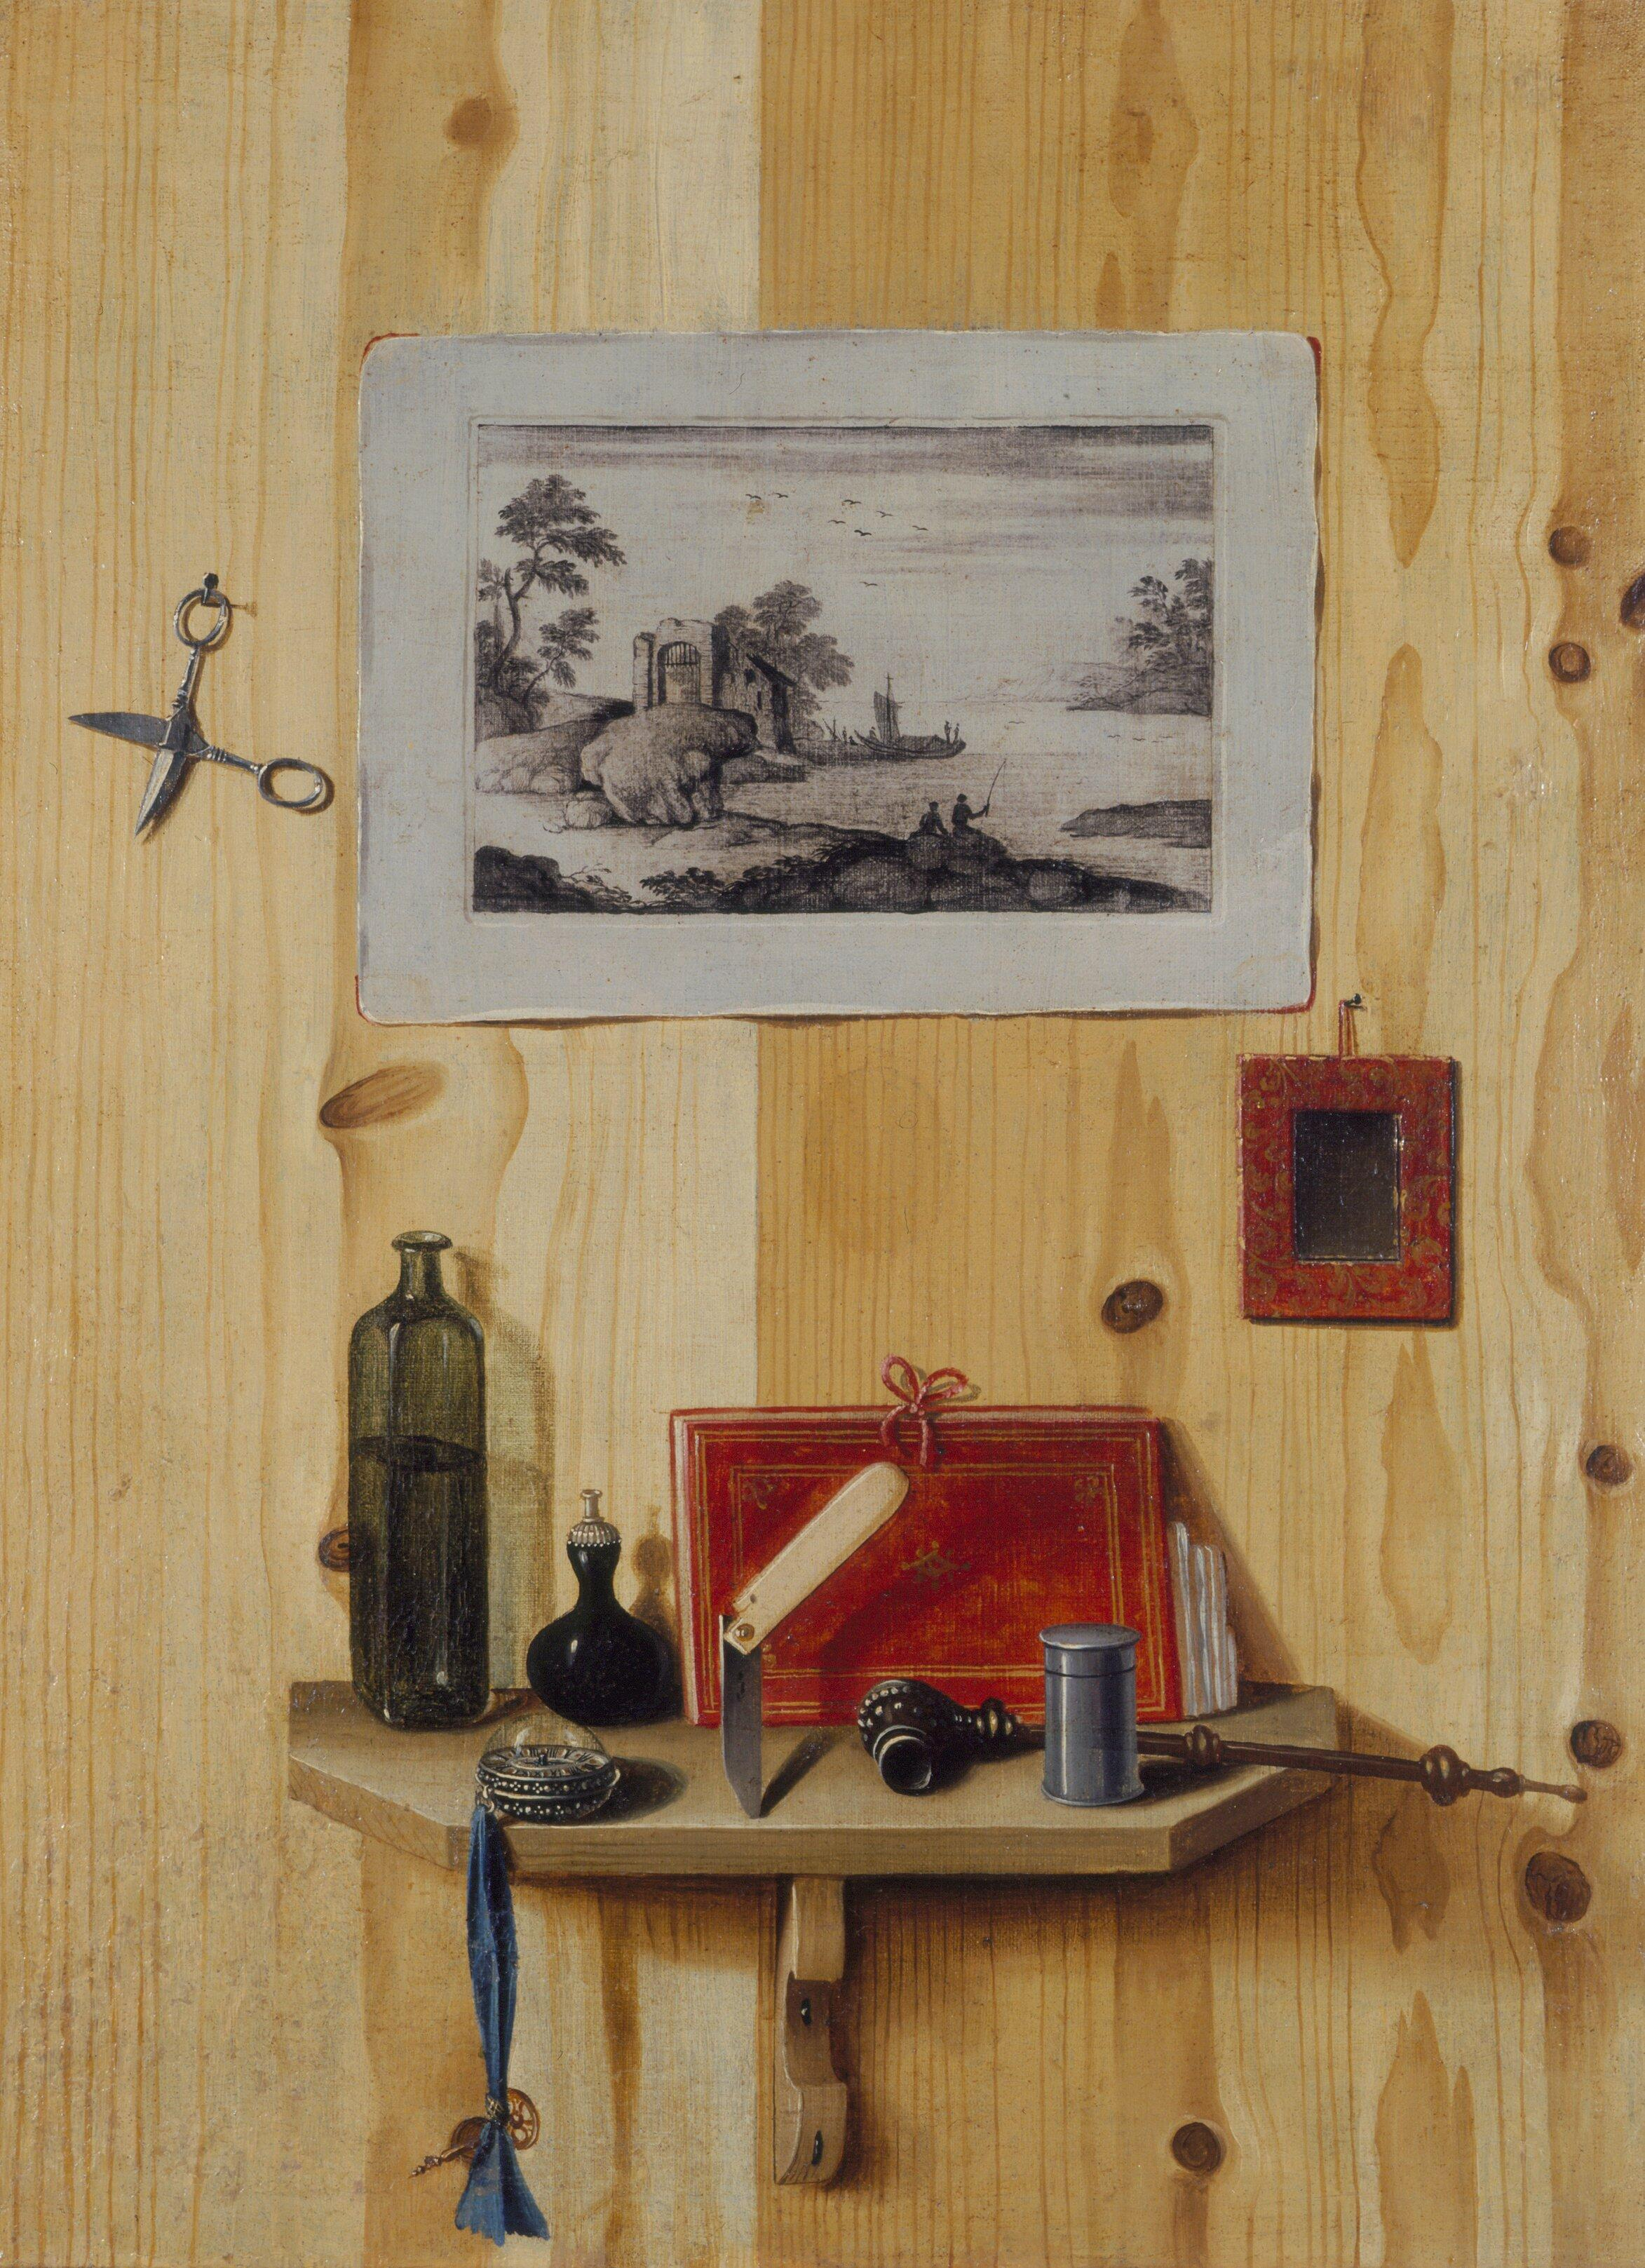
\includegraphics[scale=0.08]{Gianlisi_Antonio_Junior-Trompe_l_oeil_con_paesaggio_forbici_e_mensola_con_oggetti.jpg}}
			\bigskip
			\newline
			\begin{minipage}{0.8\linewidth}
				\centering
				Informazioni~Mancanti.
			\end{minipage}
		}
	\end{tabularx}
	}
	
	% Background image
	\AddToShipoutPictureBG*{\includegraphics[draft=false, width=\paperwidth,height=\paperheight]{example-image-plain}}
	\newpage
	
	%--------- Page 5 ----------
	
	%First line
	\begin{tabularx}{\linewidth}{XX}
		{
			
				%Scacciani Antonio - Vassoio - Rosa
				\setdf{content={\textcolor{white}{\hspace{35mm} \Large \#13}}}
				\colorbox{black}{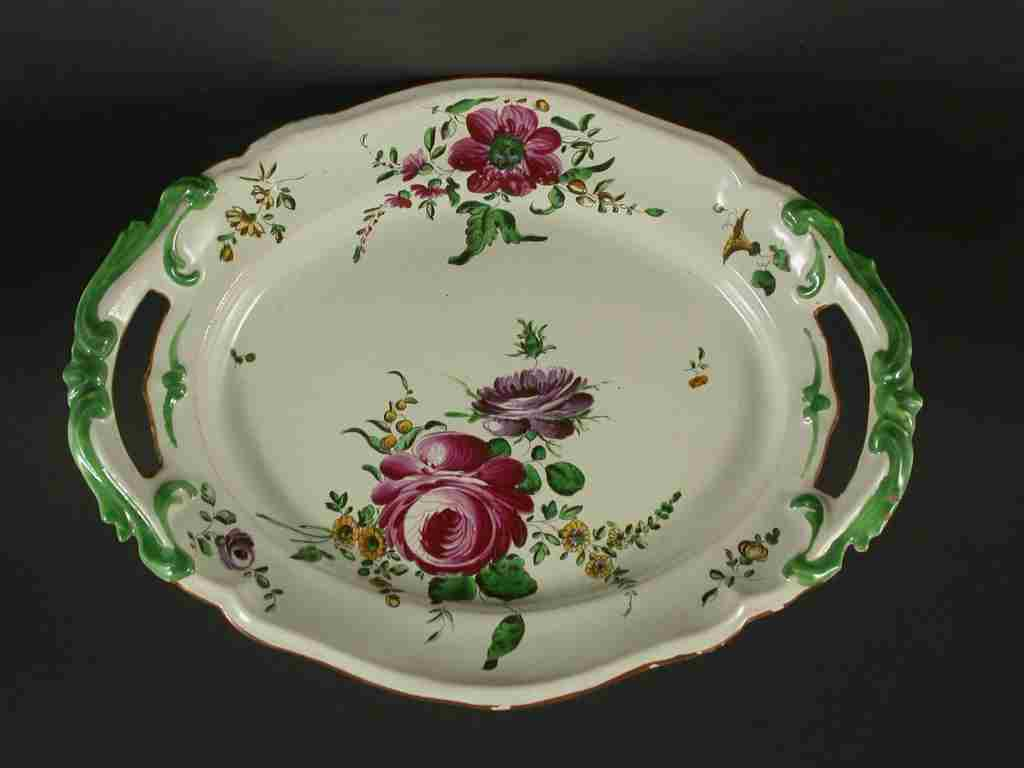
\includegraphics[]{Scacciani_Antonio-Vassoio-Rosa.jpg}}
				\bigskip
				\newline
				\begin{minipage}{0.9\linewidth}
					\raggedright
					Il Settecento è il secolo del ritorno alla natura e ai suoi valori; una ventata arcadica invade l'Europa e il decoro floreale diventa di gran moda: i fiori ornano tessuti, mobili, cornici, pareti, soffitti e ceramiche. La rosa è la protagonista del nuovo indirizzo artistico e Pesaro lega il proprio nome a questo fiore.
				\end{minipage}
		}&{
				%Realfonzo Tommaso - Natura morta con dolci frutta uova e formaggi
				\setdf{content={\textcolor{white}{\hspace{35mm} \Large \#14}}}
				\colorbox{black}{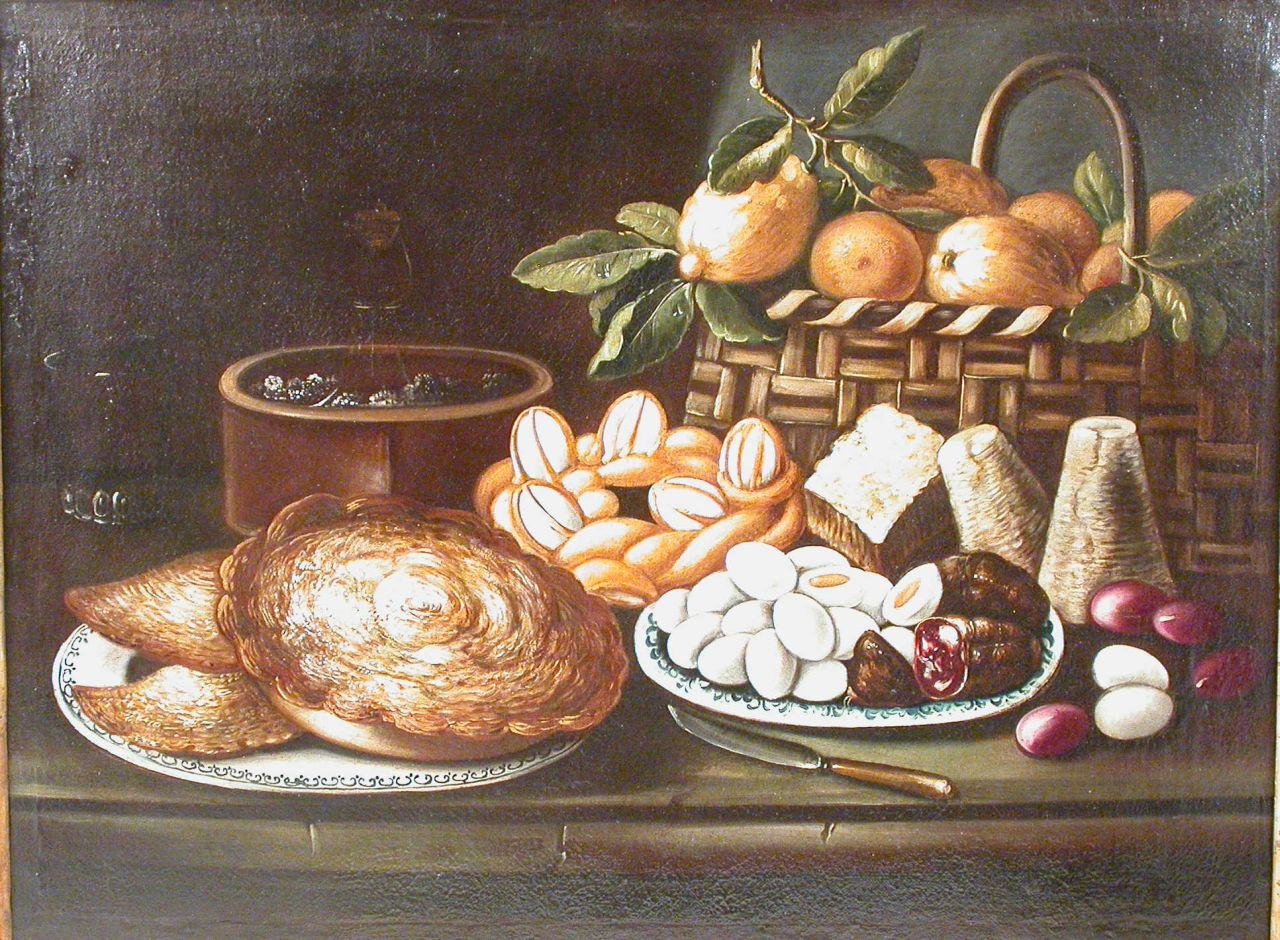
\includegraphics[scale=0.8]{Realfonzo_Tommaso-Natura_morta_con_dolci_frutta_uova_e_formaggi.jpg}}
				\bigskip
				\newline
				\begin{minipage}{0.9\linewidth}
					\raggedright
					 Il Cottino (1993), che per primo ha pubblicato questa coppia di nature morte, ne individuava correttamente la matrice partenopea, sottolineandone anche gli stretti legami con la cultura sivigliana dei bodegones. In tal senso, la sua proposta era orientata in direzione di un artista napoletano attivo nella seconda metà del seicento, seguace dello spagnolo Giovanni Quinsa.
				\end{minipage}
		}
	\end{tabularx}

	%Second line
	\vspace{5mm}
	\nopagebreak
	\begin{tabularx}{\linewidth}{X}
		\begin{center}
			
			%Gessi Giovan Francesco - Morte di Adone
			\hspace{25mm}
			\setdf{content={\textcolor{white}{\hspace{35mm} \Large \#15}}}
			\colorbox{black}{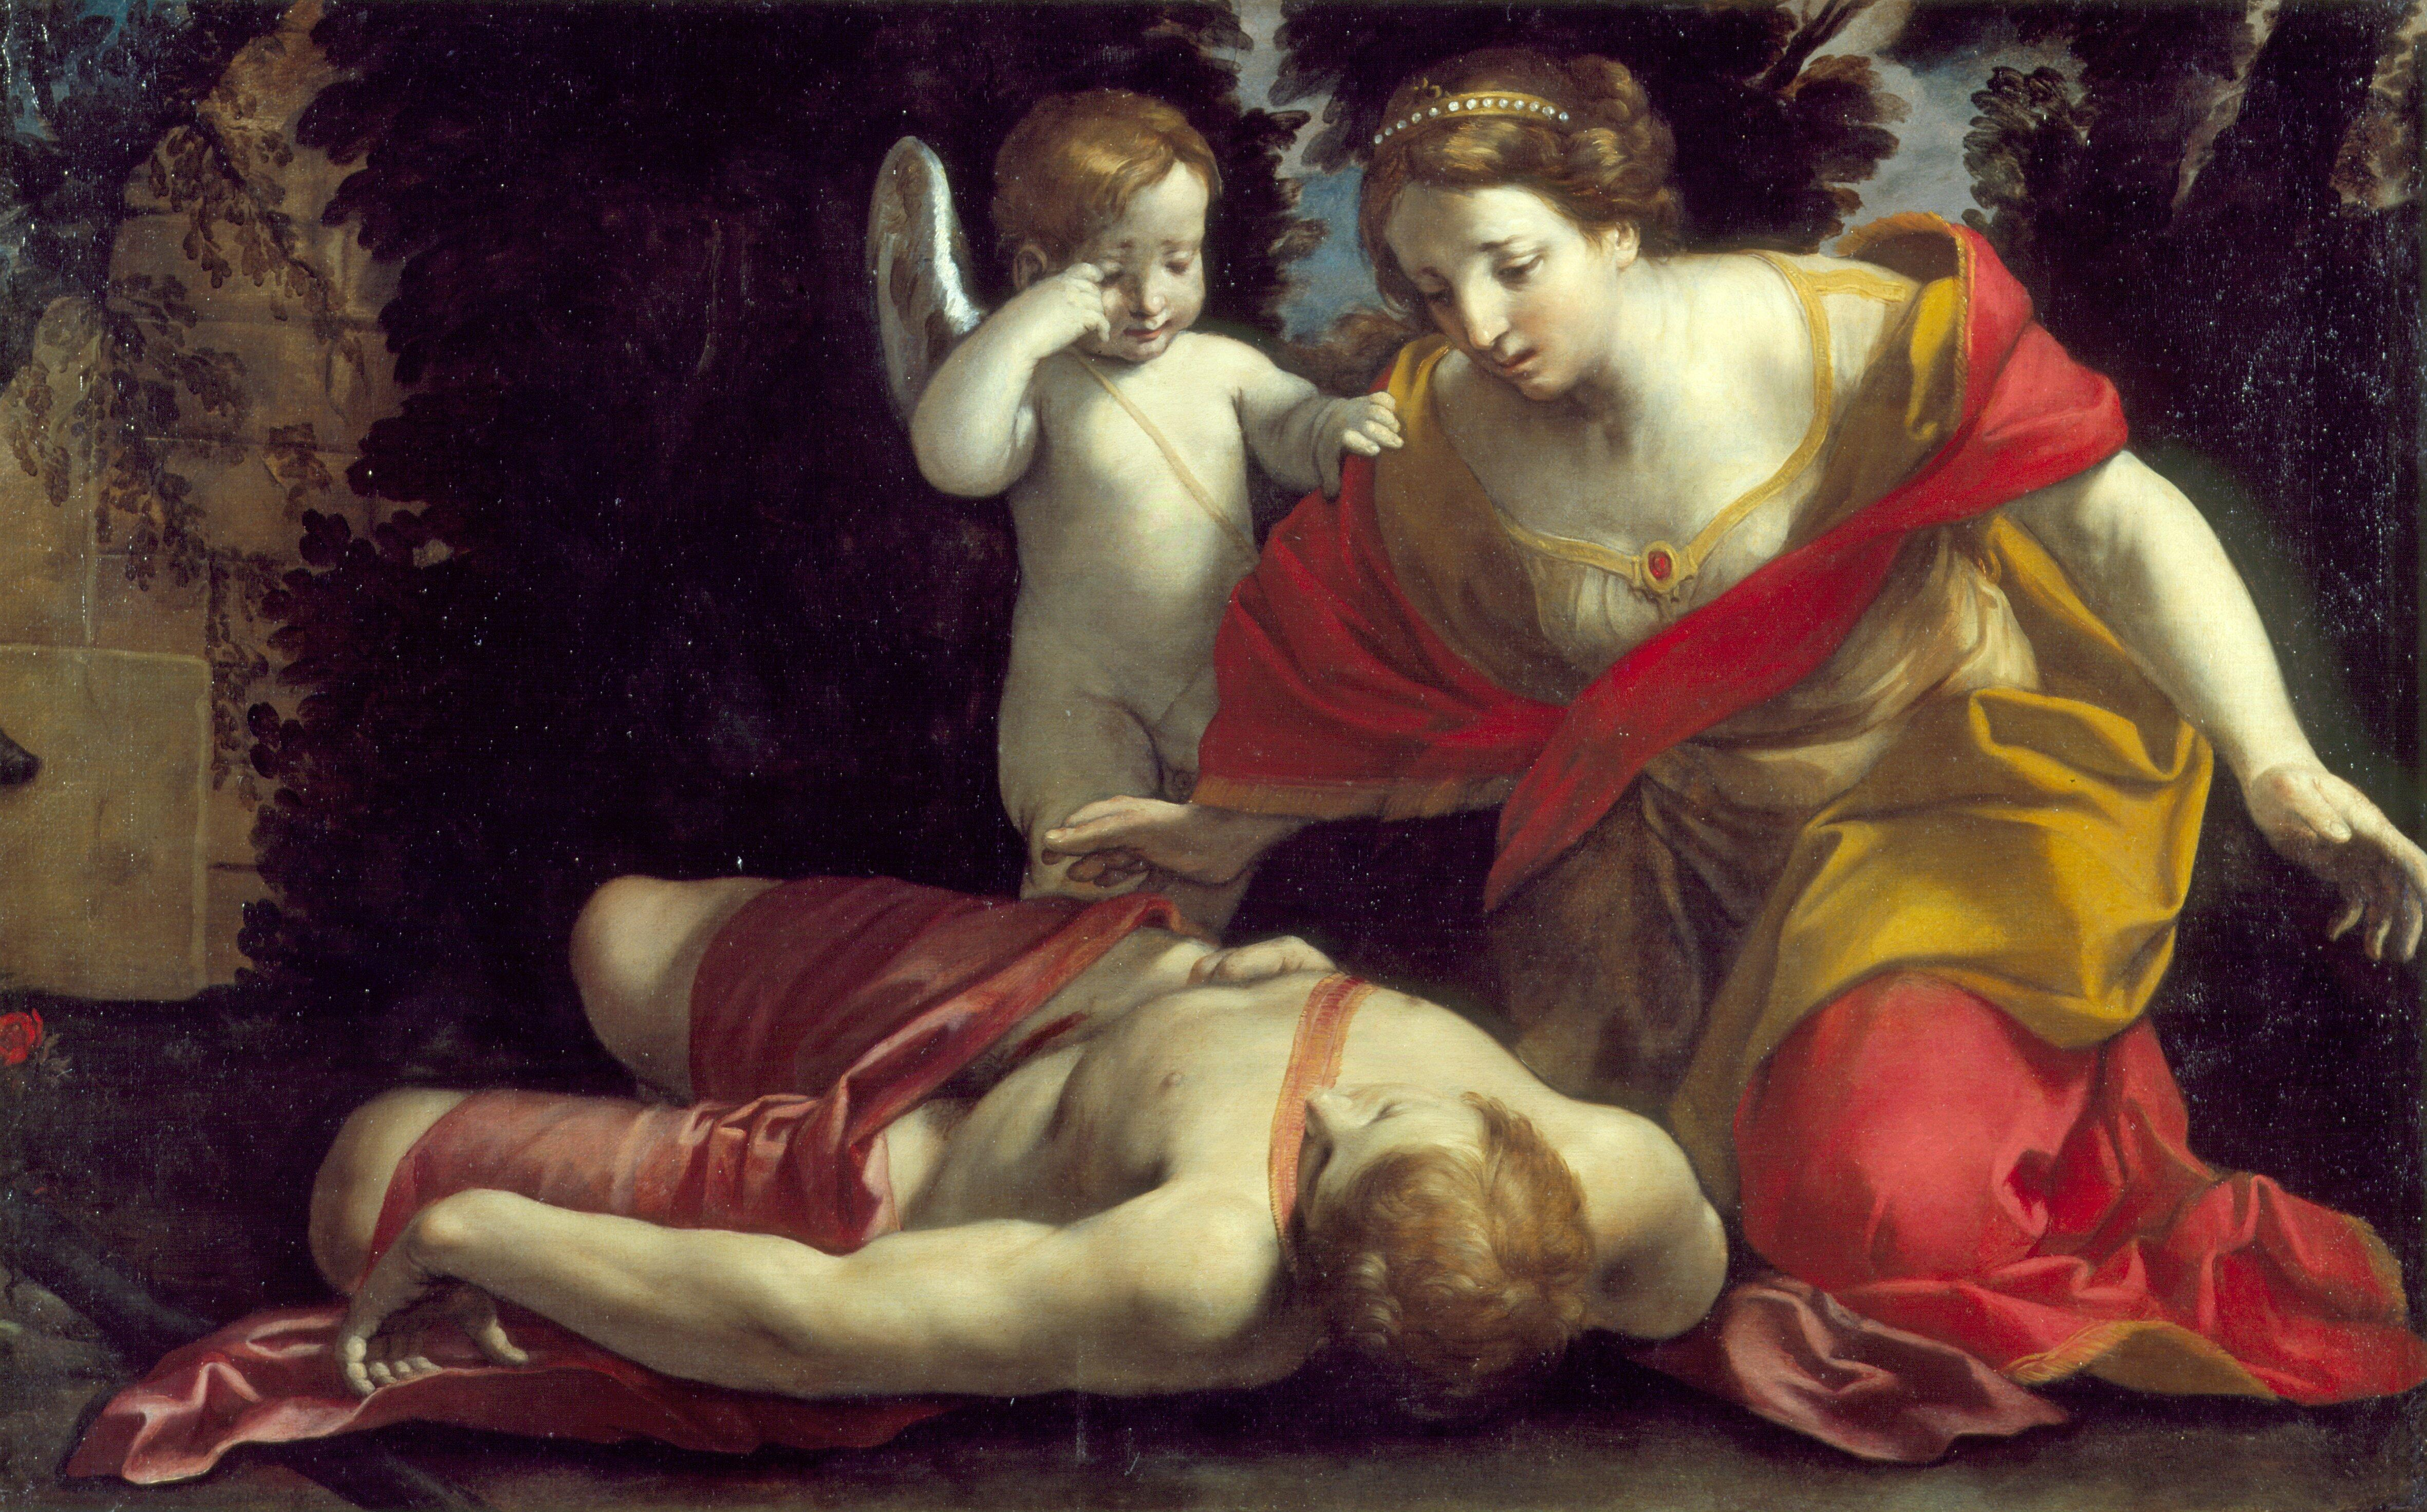
\includegraphics[scale=0.052]{Gessi_Giovan_Francesco-Morte_di_Adone.jpg}}
			\bigskip
			\newline
			\begin{minipage}{0.8\linewidth}
				\raggedright
				Sorprende nell'ultimo catalogo della Pinacoteca di Pesaro (1993) il declassamento a opera anonima di questo forte dipinto, il cui quesito attributivo risultava già ben orientato dalla precedente vicenda critica. Riferito a Giovanni Giacomo Sementi nel 1806, all'atto dell'acquisizione per via ereditaria da parte di Maria Malvezzi Hercolani ( "Adone morto, Venere e Amore che piangono, del Sementi"), e come tale ancora ricordato da Bassani (1816) e catalogato nel 1824 ("Venere, Adone, con Amorino che piange, del Sementi"), sarebbe addirittura assurto al rango di un Guido Reni nell'ultimo inventario della raccolta , risalente agli anni sessanta del XIX secolo.
			\end{minipage}
		\end{center}
	\end{tabularx}
	
	% Background image
	\AddToShipoutPictureBG*{\includegraphics[draft=false, width=\paperwidth,height=\paperheight]{example-image-plain}}
	\newpage
	
	%--------- Final page ----------
	
	\setkeys{Gin}{draft=false}
	
	\vspace*{\fill}
	\begin{center}
			\begin{minipage}{0.8\linewidth}
			\doclicenseThis
		\end{minipage}
	\end{center}
	
	% Background image
	\AddToShipoutPictureBG*{\includegraphics[draft=false, width=\paperwidth,height=\paperheight]{example-image}}
	
\end{document}
